%\chapter{Ocean Surface Modeling}
Analysis of RADAR systems in maritime environments is complicated by the fact that the ocean does not necessarily provide a smooth or uniform surface to work with. Altitude variations change the aspect angle for multipath bounces, induce wave blockage, and add clutter and spikes to the echo return \cite{skolnik_handbook}, \cite{blake_radar}, \cite{nathanson_radar}.

To capture the physical behavior of electromagnetic waves reflecting off the surface of the ocean, we need to model the surface altitude variations correctly. For this, we first need to understand the power spectra of ocean waves and their dependencies. Next, we can generate random realizations of sea surfaces by discretizing the power spectrum and taking the inverse Fourier transform of a Hermitian sequence of spectrally appropriate coefficients. This will be demonstrated in both the 1-dimensional and 2-dimensional cases.

\section {Waves in the Ocean}
Ocean waves are primarily driven by wind and start when turbulence creates capillary or surface waves with small wavelengths (on the order of a few centimeters). As the wind continues to blow, it increases both the amplitude and the wavelength of the waves until they start to interact. These interactions continue to increase the wavelength and phase speed of the waves until they are traveling faster than the wind, at which point the sea is deemed fully developed. As a sea develops, energy will transfer from higher frequencies to lower frequencies which means the power spectrum will be different for a younger sea than a mature one.

Before discussing the statistical properties of ocean waves, it is useful to review some standard nomenclature. Fetch is the length over which the wind can be considered constant, and a longer fetch generally means higher waves. Significant wave height is the mean wave height of the highest third of the waves. It is represented in the literature as $H_{1/3}$ and is equal to 4 times the standard deviation of the wave height, $H_{1/3} = 4\sigma_h$. Wave height generally refers to the mean difference between successive peaks and troughs (twice the amplitude).

\section{Ocean Wave Power Spectra}  \label{os_sec:power_spectra}
Many methods have been proposed to statistically describe the behavior of ocean waves. These range from the simplest sea state representations with a very coarse binning of wind speed and sea height variations to mathematically complex multi-parameter power spectra.

\subsection {Sea State}
The modern concept of sea state is a combination of the Beaufort wind scale and the Douglas sea scale. The Beaufort wind scale was developed in the early 1800s by sir Francis Beaufort and the Douglas sea scale was developed in the 1920s by H.P Douglas, both of the Royal Navy \cite{uk_met_fact_sheet6}. The Beaufort wind scale measures force vs. wind speed in 12 bins from "Calm" to "Hurricane" and was extended in 1944 to add scales up to 17. In 1960, it was further extended to add probable wave heights. 

The Douglas sea scale on the other hand measures sea height in 9 bins from "Calm (glossy)" to "Phenomenal". The World Meterological Organization (WMO) has adopted the Douglas sea scale as a standard \cite{wmo_code} and we can compare this to the Beaufort wind scale to add the dependency on wind speed as shown in Table \ref{os_tab:0}. There are no true standards when working with sea states, so care must be taken when comparing results between research groups.

\begin{table}[H]
  \begin{center}
      \renewcommand{\baselinestretch}{1} \small\normalsize
  \begin{quote}
    \caption[WMO Sea State vs. Wind Speed and Wave Height]{WMO Sea State vs. Wind Seed and Wave Height\label{os_tab:0}}
  \end{quote}
  \begin{tabular} {|c | c | c| c|}
    \hline
  \bf{Sea State} & \bf{Descriptio}n & \bf{Wave Height (m)} & \bf{Wind Speed (m/s)}\\ \hline
  0 & Calm (glassy) & 0 & $<$ 0.3 \\ \hline
  1 & Calm (rippled) & 0 - 0.1 & 0.3 - 1.5 \\ \hline
  2 & Smooth (wavelets) & 0.1 - 0.5 & 1.6 - 3.3 \\ \hline
  3 & Slight & 0.5 - 1.25 & 3.4 - 5.5 \\ \hline
  4 & Moderate & 1.25 - 2.5 & 5.5 - 10.7 \\ \hline
  5 & Rough & 2.5 - 4 & 10.8 - 13.8 \\ \hline
  6 & Very Rough & 4 - 6 & 13.9 - 17.1\\ \hline
  7 & High & 6 - 9 & 17.2 - 24.4\\ \hline
  8 & Very High & 9 - 14 & 24.5 - 32.6\\ \hline
  9 & Phenomenal & $\geq$ 14 & $\geq$ 32.7\\ \hline
\end{tabular}
\end{center}
\end{table}
\renewcommand{\baselinestretch}{2} \small\normalsize

\subsection{Pierson-Moskowitz Spectrum}
In 1964, the Pierson-Moskowitz (PM) spectrum given in Equation \ref{os_eq:1} was developed to describe the power spectrum of the variance of wave height in terms of the measured wind speed 19 meters above the sea surface ($U_{19}$) \cite{michel_sea_spectra}. 
 \begin{equation}
S(k) = \frac{0.0081}{k^3}e^{-0.74\left(\frac{g}{k}\right)^2U_{19}^{-4}}
\label{os_eq:1}
\end{equation}
 \renewcommand{\baselinestretch}{2} \small\normalsize
Here, $g$ is the coefficient of gravity ($g = 9.81 m/s^2$). 
 
The PM spectrum is a single parameter spectrum as wind speed only drives the exponential term of Equation \ref{os_eq:1}. The variance power spectrum is shown in the left hand side of Figure \ref{os_fig:1} and the associated curvature spectrum is shown in the right hand side of Figure \ref{os_fig:1}, both for wind speeds from 3 m/s to 21 m/s in increments of 2 m/s. The curvature spectrum is also referred to as the saturation spectrum. It removes the $k^{-3}$ dependence of the power spectrum and allows high spatial frequency behavior to be more readily observed.
 
 \begin{figure}[H]
  \begin{center}
\includegraphics[width=6in]{../media/Ocean_Surface/PM_variance_curvature_spectrum.png}
  \end{center}
  \renewcommand{\baselinestretch}{1} \small\normalsize
  \begin{quote}
    \caption[Pierson-Moskowitz Variance and Curvature Spectra]{Pierson-Moskowitz Variance and Curvature Spectra\label{os_fig:1}}
  \end{quote}
\end{figure}
 \renewcommand{\baselinestretch}{2} \small\normalsize
From Figure \ref{os_fig:1} we can see that, for the PM spectrum, wind speed impacts the spectral peak and low spatial frequency cutoff but has no effect at high spatial frequencies.
 
The PM spectrum assumes deep water, infinite fetch and no swells and has repeatedly been shown to be accurate for gravity waves in fully developed seas, but fails to capture spectral peaks due to high winds over short fetches.

\subsection{Bretschneider Spectrum}
To overcome the limitations of a spectrum that requires fully developed seas, several multi-parameter spectra have been developed. In 1978, the 12th International Towing Tank Conference recommended the Bretschneider spectrum \cite{michel_sea_spectra} shown in Equation \ref{os_eq:1a} where the modal frequency $\omega_m$ is given by $\omega_m = 0.4\sqrt{g/H_{1/3}}$.
\begin{equation}
  \begin{gathered}
  \label{os_eq:1a}
  S(k) = \frac{1.25 \omega_m^4}{8k^3g^2}e^{-1.25\frac{\omega_m^4}{g^2k^2}} 
  \end{gathered}
\end{equation}
\renewcommand{\baselinestretch}{2} \small\normalsize
Figure \ref{os_fig:1a} shows the variance power spectrum on the left hand side and the associated curvature spectrum on the right hand side, both for wave height standard deviations from 0.1 m to 1 m in increments of 0.1 m.

 \begin{figure}[H]
  \begin{center}
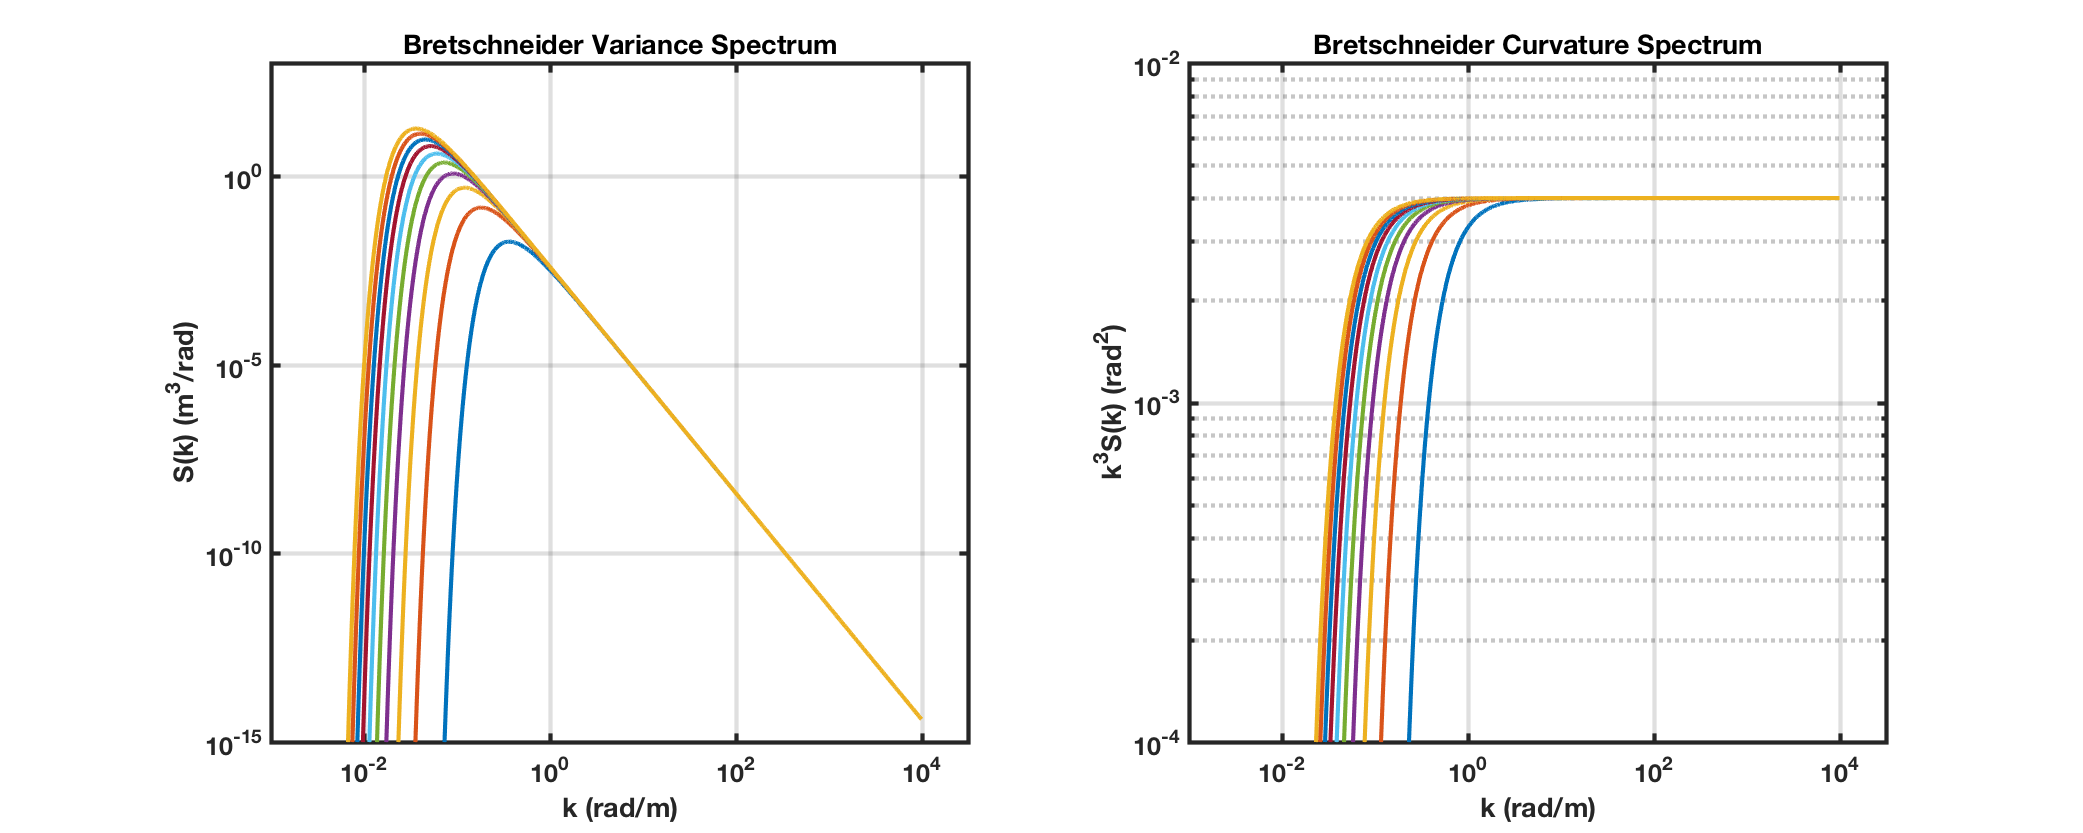
\includegraphics[width=6in]{../media/Ocean_Surface/bs_variance_curvature_spectrum.png}
  \end{center}
  \renewcommand{\baselinestretch}{1} \small\normalsize
  \begin{quote}
    \caption[Bretschneider Variance and Curvature Spectra]{Bretschneider Variance and Curvature Spectra\label{os_fig:1a}}
  \end{quote}
\end{figure}
 \renewcommand{\baselinestretch}{2} \small\normalsize
The Bretschneider spectrum is a two-parameter spectrum as both the exponential term and the amplitude in Equation \ref{os_eq:1a} are dependent on significant wave height.

\subsection{JONSWAP Spectrum}
The Joint North Sea Wave Project (JONSWAP) in the 1970s modified the Pierson-Moskowitz spectrum by adding a peak enhancement factor as shown in Equation \ref{os_eq:1b} \cite{michel_sea_spectra}.
\begin{equation}
  \label{os_eq:1b}
  S(k) = S_{PM}(k)\nu^{\frac{k-k_0}{2\sigma^2k_0}} 
  \end{equation}
The enhancement factor $\nu$ was empirically derived for locations in the North Sea and allows control of the amplitude as in the Bretschneider spectrum. The difference is that the JONSWAP enhancement factor only amplifies the spectrum around the spectral peak.

\subsection{Elfouhaily Spectrum}
Many additional spectra have been developed and in 1997, Elfouhaily et. al extended several of these to provide a unified modern spectrum that is broken into low and high spatial frequency regions, $B_l$ and $B_h$, \cite{elfouhaily}. 

\subsubsection{Spectrum Definition}
The 1-dimensional version of the Elfouhaily spectrum is given in Equation \ref{os_eq:2}.
\begin{equation}
  \label{os_eq:2}
  S(k) = k^{-3}\left[B_l + B_h \right]
\end{equation}
\renewcommand{\baselinestretch}{2} \small\normalsize
This spectrum is dependent on the wind speed at 10 m altitude ($U_{10}$) and the inverse age parameter ($\Omega$). The inverse age parameter indicates how developed the sea is; fully developed for $\Omega = 0.84$, mature for $\Omega = 1.0$, and young for $\Omega > 2.0$. 

The low spatial frequency region, $B_l$, is given by Equation \ref{os_eq:3} and the parameters are defined in Table \ref{os_tab:1} and Equation \ref{os_eq:3a}. Here we are using $v$ to represent phase speed rather than $c$ to prevent confusion with the speed of light.
\begin{equation}
  \label{os_eq:3}
 B_l = \frac{1}{2} \alpha_p \frac{v_p}{v} F_p
\end{equation}
\renewcommand{\baselinestretch}{2} \small\normalsize
\begin{subequations}
\label{os_eq:3a}
   Low spatial frequency spectrum dependencies:
\begin{align}
  F_p &= L_{PM}J_pe^{-\frac{\Omega}{\sqrt{10}}\left[\sqrt{k/_{k_p}} - 1 \right]} &  k_p &= g\left(\frac{\Omega}{U_{10}}\right)^2 & v_p &= \frac{U_{10}}{\Omega} \\
   L_{PM} &=e^{-\frac{5}{4}\left(\frac{k_p}{k} \right)^2} &  J_p &= \gamma^\Gamma  & \alpha_p &= 0.006\Omega^{0.55} 
\end{align}
\end{subequations}
\renewcommand{\baselinestretch}{2} \small\normalsize
\begin{table}[H]
  \begin{center}
      \renewcommand{\baselinestretch}{1} \small\normalsize
  \begin{quote}
    \caption[Elfouhaily Low Spatial Frequency Spectrum Parameters]{Elfouhaily Low Spatial Frequency Spectrum Parameters\label{os_tab:1}}
  \end{quote}
  \begin{tabular} {|c | c |}
    \hline
  \bf{Parameter} & \bf{Description} \\ \hline
  $F_p$ & Long wave side effect function \\ \hline
  $k_p$ &  Wave number of the spectral peak \\ \hline
  $v_p$ &  Phase speed at the spectral peak \\ \hline
  $L_{PM}$ & PM shape spectrum \\ \hline
  $J_p$ & JONSWAP peak enhancement function \\ \hline
  $\alpha_p$ & Generalized Phillips-Kitaigorodskii long wave equilibrium range parameter\\ \hline
  $v$ & Phase speed of the wave \\ \hline
\end{tabular}
\end{center}
\end{table}
\renewcommand{\baselinestretch}{2} \small\normalsize
The high spatial frequency region, $B_h$, is given by Equation \ref{os_eq:4} and the parameters are defined in Table \ref{os_tab:2} and Equations \ref{os_eq:4a} and \ref{os_eq:4b}.
\begin{equation}
  \label{os_eq:4}
 B_h = \frac{1}{2} \alpha_m \frac{v_m}{v} F_m
\end{equation}
\renewcommand{\baselinestretch}{2} \small\normalsize
\begin{subequations}
\label{os_eq:4a}
   High spatial frequency spectrum dependencies:
\begin{align}
  F_m &= L_{PM}J_pe^{-\frac{1}{4}\left[k/_{k_m} - 1 \right]^2 } & k_m & = 370 \text{ rad/m} &  v_m &=\sqrt{\frac{2g}{k_m}} = 0.23 \text{ m/s} \\
  u^* &= \sqrt{Cd_{10N}}U_{10}  & L_{PM} &=e^{-\frac{5}{4}\left(\frac{k_p}{k} \right)^2}  &  J_p &= \gamma^\Gamma
\end{align}
\end{subequations}
\renewcommand{\baselinestretch}{2} \small\normalsize
\begin{equation}
\begin{gathered}
  \label{os_eq:4b}
   \alpha_m= \begin{cases}
    10^{-2}\left[1 + \log\left(\frac{u^*}{v_m} \right) \right],& \text{if } u^* \leq v_m\\
    10^{-2}\left[1 + 3\log\left(\frac{u^*}{v_m} \right) \right], & \text{if } u^* > v_m\\
  \end{cases}
\end{gathered}
\end{equation}
\renewcommand{\baselinestretch}{2} \small\normalsize

\begin{table}[H]
  \begin{center}
      \renewcommand{\baselinestretch}{1} \small\normalsize
  \begin{quote}
    \caption[Elfouhaily High Spatial Frequency Spectrum Parameters]{Elfouhaily High Spatial Frequency Spectrum Parameters\label{os_tab:2}}
  \end{quote}
  \begin{tabular} {|c | c |}
    \hline
  \bf{Parameter} & \bf{Description} \\ \hline
  $F_m$ & Short wave side effect function \\ \hline
  $k_m$ &  Wave number at the secondary peak of the curvature spectrum \\ \hline
  $v_m$ &  Minimum phase speed at $k_m$ \\ \hline
  $\alpha_m$ & Generalized Phillips-Kitaigorodskii short wave equilibrium range parameter \\ \hline
  $L_{PM}$ & PM shape spectrum \\ \hline
  $J_p$ & JONSWAP peak enhancement function \\ \hline
  $Cd_{10N}$ & Neutral stability drag coefficient at 10 m above sea level, $\approx 0.00144$ \\ \hline
  $u^*$ & Friction velocity at the water surface \\ \hline
  $v$ & Phase speed of the wave \\ \hline
\end{tabular}
\end{center}
\end{table}
\renewcommand{\baselinestretch}{2} \small\normalsize
The variables $L_{PM}$ and $J_p$ are found in both $B_l$ and $B_h$ and are given by Equation \ref{os_eq:5}.
\begin{equation}
\begin{gathered}
  \label{os_eq:5}
    \gamma = \begin{cases}
    1.7,& \text{if } 0.84 < \Omega < 1\\
    1.7 + 6\log{\Omega}, & \text{if } 1 < \Omega < 5
  \end{cases} \\
  \Gamma = \exp{\left[- \frac{\left(\sqrt{\frac{k}{kp} - 1} \right)^2}{2\sigma^2} \right]} \\
  \sigma = 0.08\left[1 + 4\Omega^{-3} \right] \\
\end{gathered}
\end{equation}
\renewcommand{\baselinestretch}{2} \small\normalsize
In \cite{elfouhaily}, the dispersion relation that holds for both gravity and capillary waves is given as 
\begin{equation}
\label{os_eq:5aa}
\omega^2 = gk\left[1 + \left(\frac{k}{k_m}\right)^2 \right]
\end{equation}
We can use Equation \ref{os_eq:5aa} to define the phase speed as
\begin{equation}
\label{os_eq:5ab}
v = \frac{\omega}{k}= \sqrt{\frac{g}{k}\left[1 + \left(\frac{k}{k_m}\right)^2 \right]}
\end{equation}

In the case where we have fetch rather than the inverse age parameter, we can compute the inverse age parameter as shown in Equation \ref{os_eq:5a}. Here $x$ is the dimensional fetch in m and $X$ is the non-dimensional fetch.
\begin{equation}
\label{os_eq:5a}
\begin{gathered}
 X = \frac{g}{U_{10}^2}x\\
 X_0 = 2.2 \times 10^4 \\
 \Omega = 0.84\tanh\left[\left(\frac{X}{X_0} \right)^{0.4} \right]^{-0.75} \\
\end{gathered}
\end{equation}
\renewcommand{\baselinestretch}{2} \small\normalsize

\subsubsection{1-Dimensional Spectrum Visualization}
Figure \ref{os_fig:3} shows the variance power spectrum is shown on the left hand side and the associated curvature spectrum is shown on the right hand side. These figures were generated for wind speeds from 3 m/s to 21 m/s in increments of 2 m/s, matching Figure 8 in \cite{elfouhaily}. In these figures, the secondary peak can clearly be seen at 370 rad/m.
\begin{figure}[H]
  \begin{center}
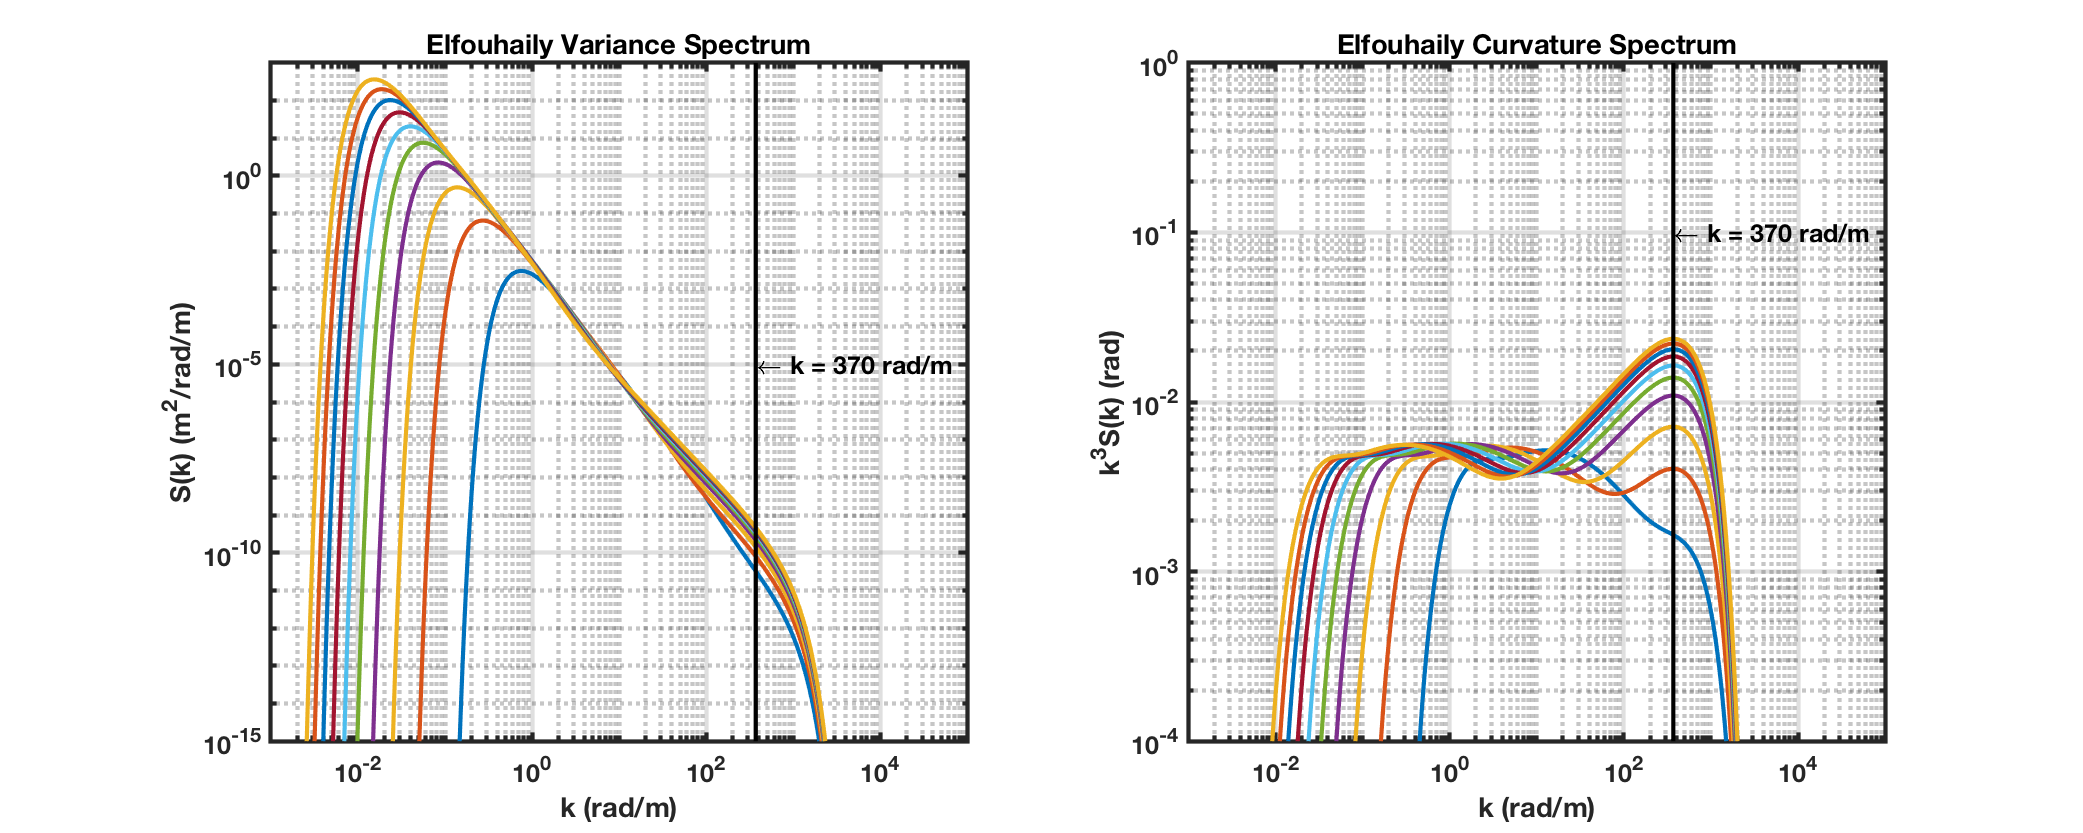
\includegraphics[width=6in]{../media/Ocean_Surface/elf_variance_curvature_spectrum.png}
  \end{center}
  \renewcommand{\baselinestretch}{1} \small\normalsize
  \begin{quote}
    \caption[Elfouhaily Variance and Curvature Spectra vs. $U_{10}$]{Elfouhaily Variance and Curvature Spectra vs. $U_{10}$\label{os_fig:3}}
  \end{quote}
\end{figure}
\renewcommand{\baselinestretch}{2} \small\normalsize

To demonstrate the impact of the inverse age parameter, Figure \ref{os_fig:3a} shows the variance power spectrum on the left hand side and the associated curvature spectrum on the right hand side. These figures were generated for $\Omega$ ranging from $0.84$ (fully developed) to $5.0$ (very young). From this figure, we can see that the spectra show energy transferring from high spatial frequencies to low spatial frequencies and the spectral peak flattening as the sea develops.
\begin{figure}[H]
  \begin{center}
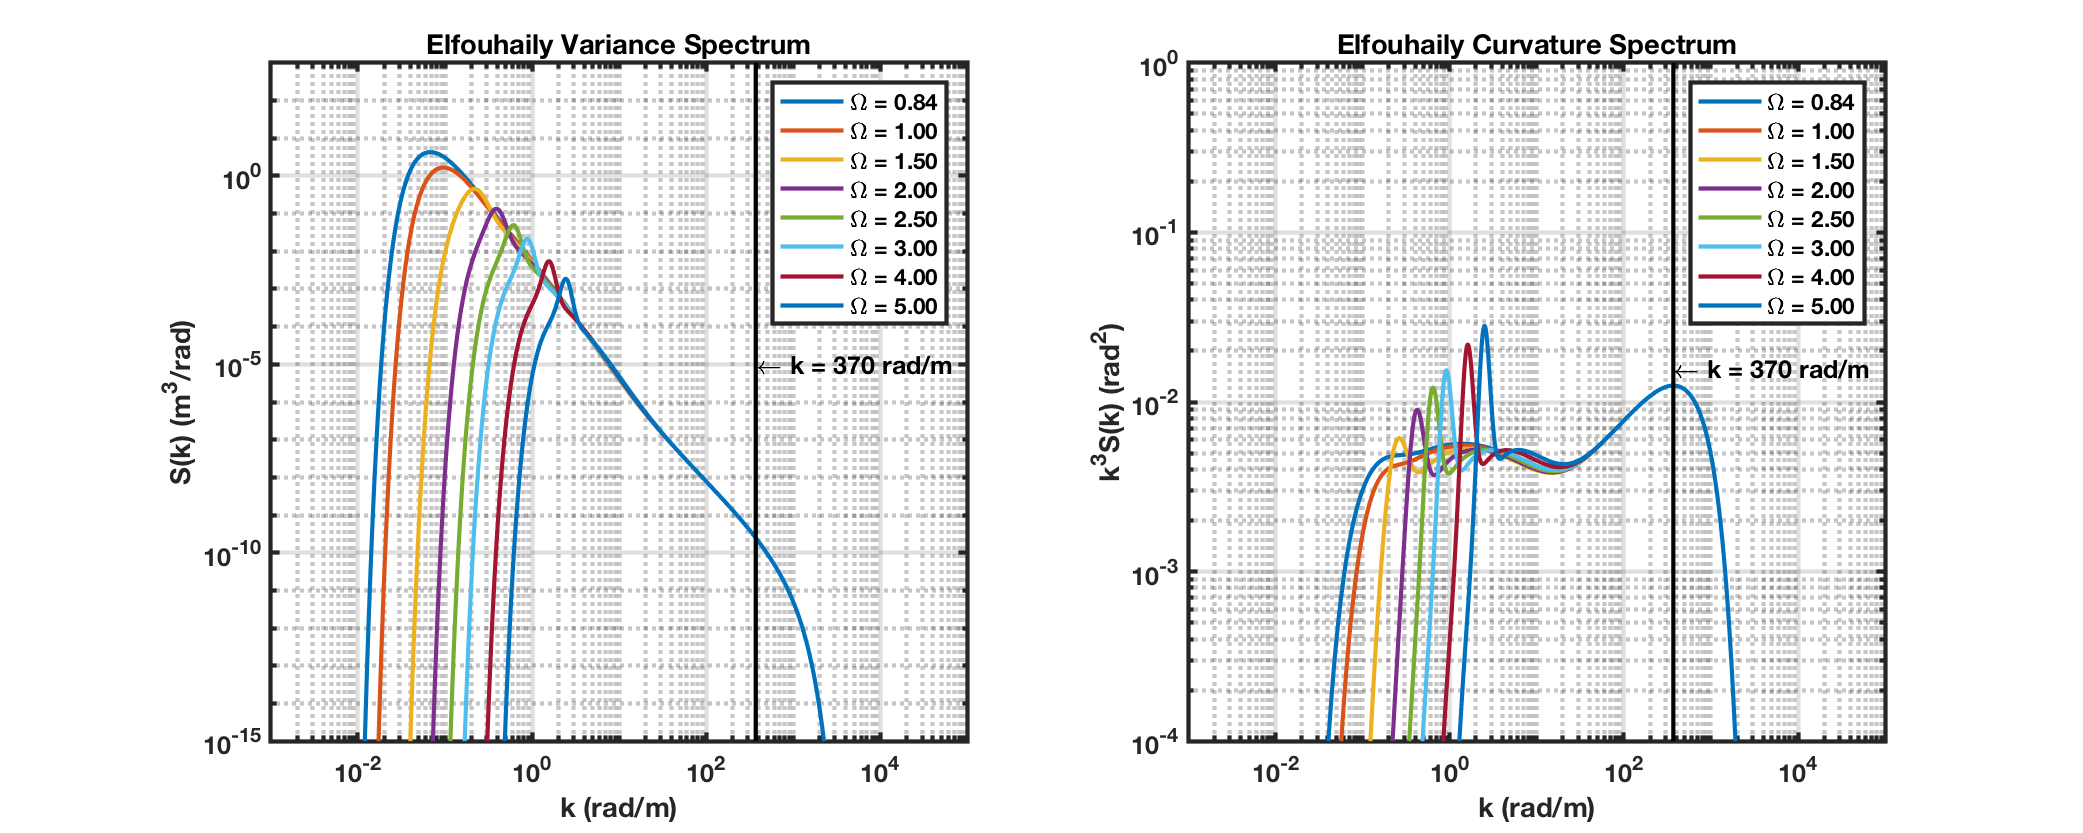
\includegraphics[width=6in]{../media/Ocean_Surface/elf_variance_curvature_spectrum_age.png}
  \end{center}
  \renewcommand{\baselinestretch}{1} \small\normalsize
  \begin{quote}
    \caption[Elfouhaily Variance and Curvature Spectra vs. $\Omega$]{Elfouhaily Variance and Curvature Spectra vs. $\Omega$ \label{os_fig:3a}}
  \end{quote}
\end{figure}
\renewcommand{\baselinestretch}{2} \small\normalsize

\subsubsection{Comparison with PM Spectrum}
As a comparison, the Elfouhaily and PM variance power spectra are shown in the left hand side of Figure \ref{os_fig:2} for wind speeds of 5 m/s and 10 m/s. The inverse age parameter was set to 0.84 to match and the wind speed at 19 m altitude was approximated as $U_{19} \approx 1.026 U_{10}$. The Elfouhaily spectra are shown by the dashed lines and indicate a deviation from the PM spectra at large wave numbers. The corresponding curvature spectra are shown in the right hand side of Figure \ref{os_fig:2}. 
\begin{figure}[H]
  \begin{center}
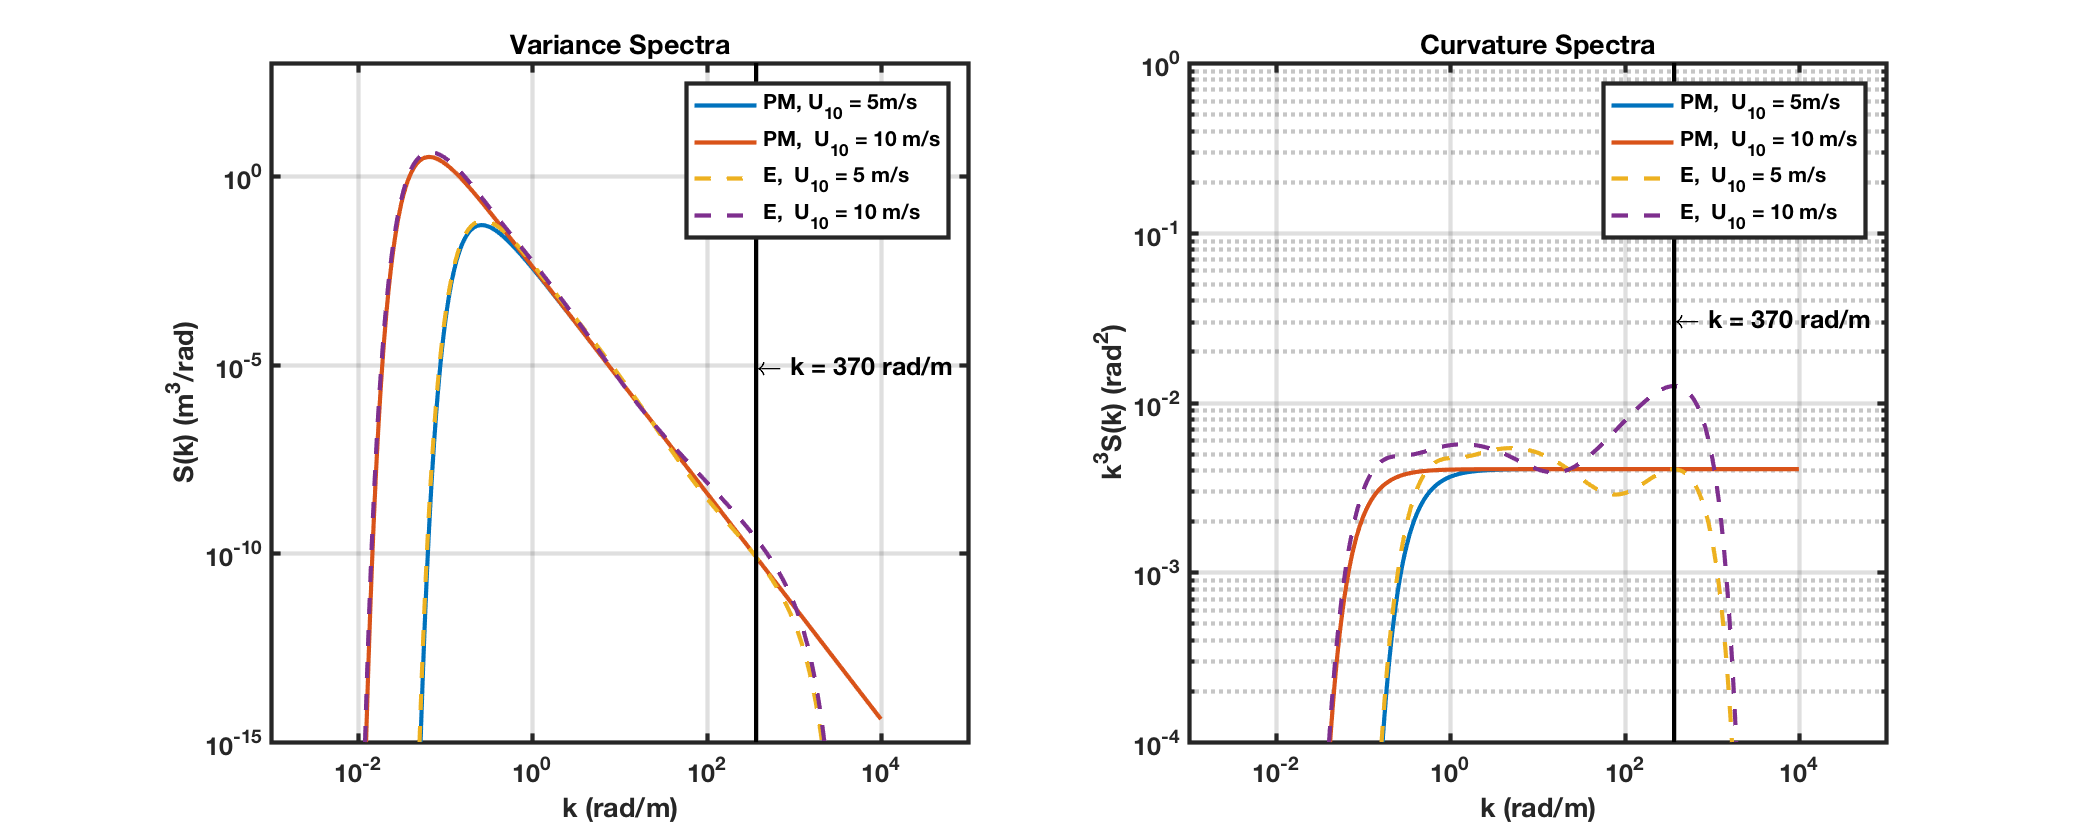
\includegraphics[width=6in]{../media/Ocean_Surface/elf_vs_PM_variance_curvature_spectrum.png}
  \end{center}
  \renewcommand{\baselinestretch}{1} \small\normalsize
  \begin{quote}
    \caption[Elfouhaily vs. Pierson Moskowitz Variance and Curvature Spectra]{Elfouhaily vs. Pierson Moskowitz Variance and Curvature Spectra\label{os_fig:2}}
  \end{quote}
\end{figure}
\renewcommand{\baselinestretch}{2} \small\normalsize

\subsubsection{Directional Spreading Functions}
All the variance power spectra that have been discussed are uni-directional, meaning they only apply downrange in the direction of the wind. For two-dimensional surfaces, we need to include angular extent. This can be accomplished by applying a spreading function $\Phi$ in $k$-space as shown in Equation \ref{os_eq:5b} \cite{elfouhaily}.
\begin{equation}
\label{os_eq:5b}
\Psi(k,\phi) = \frac{1}{k}S(k)\Phi(k,\phi)
\end{equation}
\renewcommand{\baselinestretch}{2} \small\normalsize
As discussed in \cite{elfouhaily}, the spreading function should be symmetric in downwind-crosswind and will have the form given in Equation \ref{os_eq:5c}.
\begin{equation}
\label{os_eq:5c}
\Psi(k,\phi) = \frac{1}{2\pi}\left[1 + \Delta(k)\cos(2\phi) \right]
\end{equation}
\renewcommand{\baselinestretch}{2} \small\normalsize

Here $\Delta(k)$ is defined as in Equation \ref{os_eq:5d}.
\begin{equation}
\label{os_eq:5d}
\begin{gathered}
\Delta(k) = \tanh\left( a_0 + a_p\left(\frac{v}{v_p}\right)^{2.5}  + a_m\left(\frac{v_m}{v} \right)^{2.5}\right)\\
a_0 = \frac{\log(2)}{4} \\
a_p = 4\\
a_m = 0.13\frac{u^*}{v_m} \\
\end{gathered}
\end{equation}
\renewcommand{\baselinestretch}{2} \small\normalsize

In Equation \ref{os_eq:5c}, $\phi$ is the azimuth angle in the $x$-$y$ plane, so that the downwind direction will be along the positive $x$-axis and the crosswind direction will be along the positive $y$-axis. The true orientation of these axes is arbitrary and can be rotated to any desired coordinate frame.

The complete 2-dimensional unified Elfouhaily spectrum is given in Equation \ref{os_eq:5e}.
\begin{equation}
\label{os_eq:5e}
\boxed{\Psi(k,\phi) = \frac{1}{2\pi k^4}\left[B_l + B_h \right] \left[1 + \Delta(k)\cos(2\phi) \right]}
\end{equation}

\subsubsection{2-Dimensional Spectrum Visualization}
Figure \ref{os_fig:7bb} shows the 2-D variance and curvature power spectra. In the curvature spectrum, we can see the secondary peak along the $x$-axis as in the 1-dimensional case. The secondary peak is not observed along the $y$-axis as that represents the crosswind direction where additional energy is not being injected by the wind.
\begin{figure}[H]
  \begin{center}
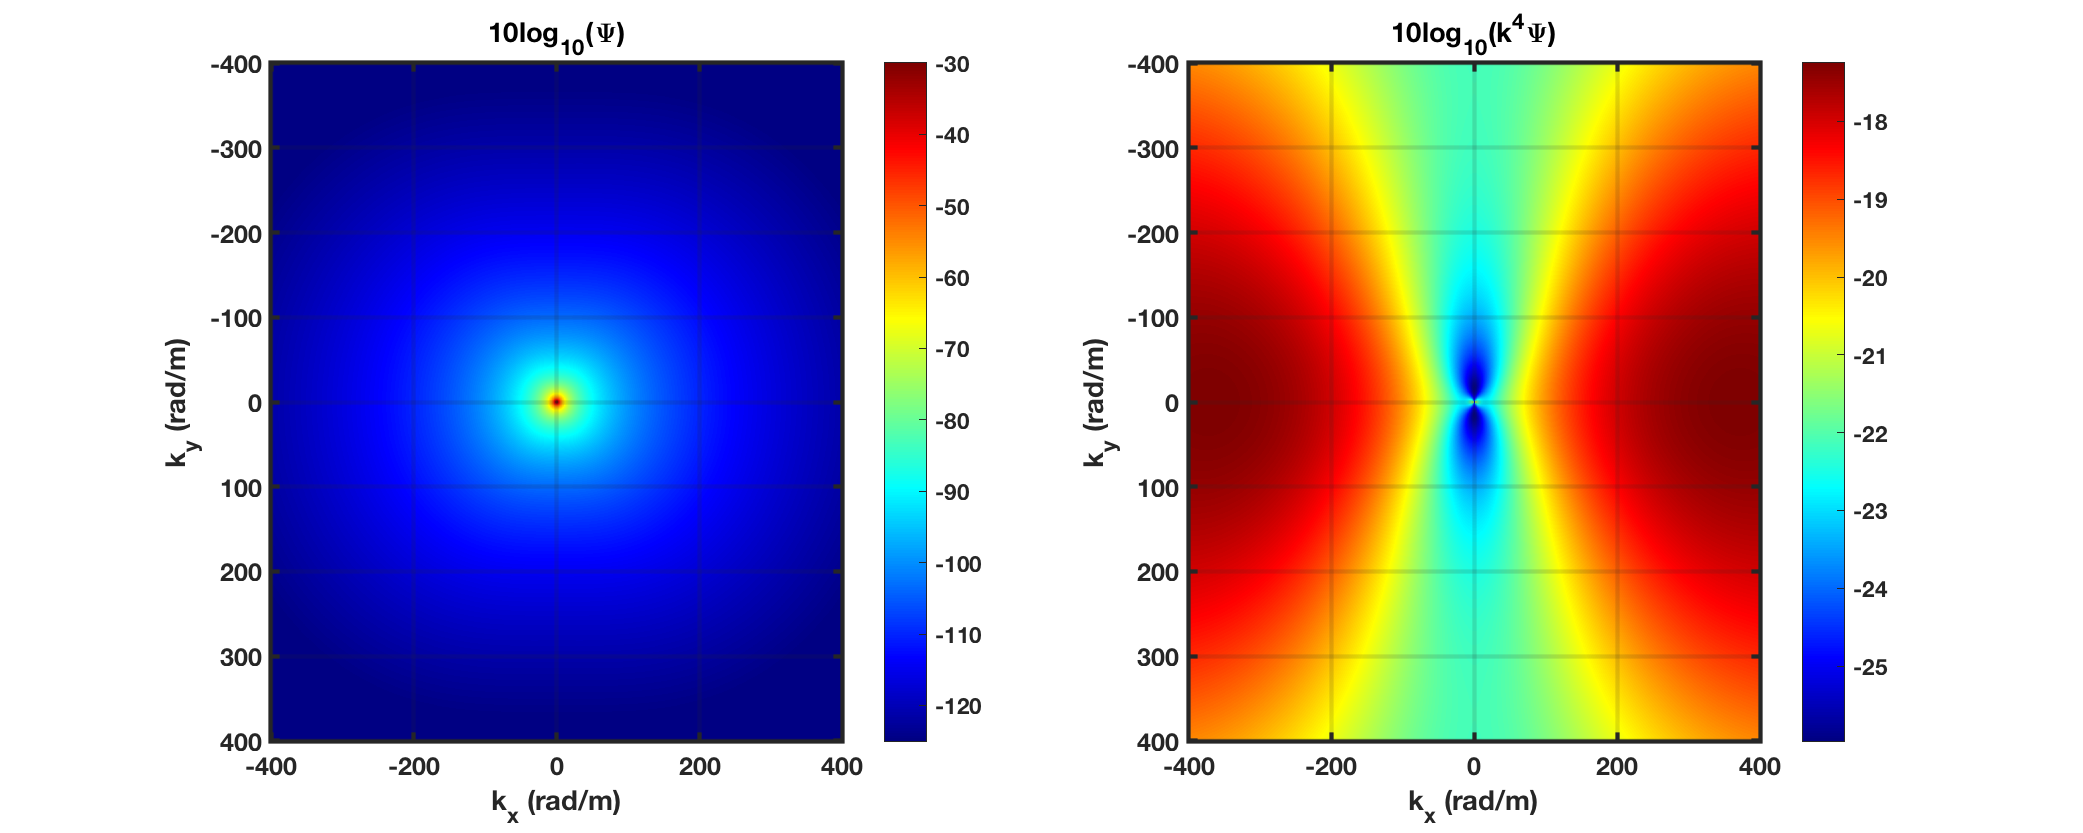
\includegraphics[width=6in]{../media/Ocean_Surface/elf_variance_curvature_spectrum_2D.png}
  \end{center}
  \renewcommand{\baselinestretch}{1} \small\normalsize
  \begin{quote}
    \caption[Elfouhaily 2-D Variance and Curvature Power Spectra]{Elfouhaily 2-D Variance and Curvature Power Spectra\label{os_fig:7bb}}
  \end{quote}
\end{figure}
\renewcommand{\baselinestretch}{2} \small\normalsize

Figure \ref{os_fig:7bc} shows 2-D slices of the power spectrum vs the 1-D power spectrum on the left hand side and the same for the curvature spectrum on the right hand side, where $\Psi_x = \Psi(k_y = 0)$ and $\Psi_y = \Psi(k_x = 0)$. The 2-D spectral slices are plotted as $k_x\Psi_x$ and $k_y\Psi_y$ so that all three spectra have the same units. Note that the $\Psi_x$ slice $\approx S$ and that the $\Psi_y$ slice has a shifted spectral peak and low frequency cutoff but converges to the other spectra at high spatial frequencies.
\begin{figure}[H]
  \begin{center}
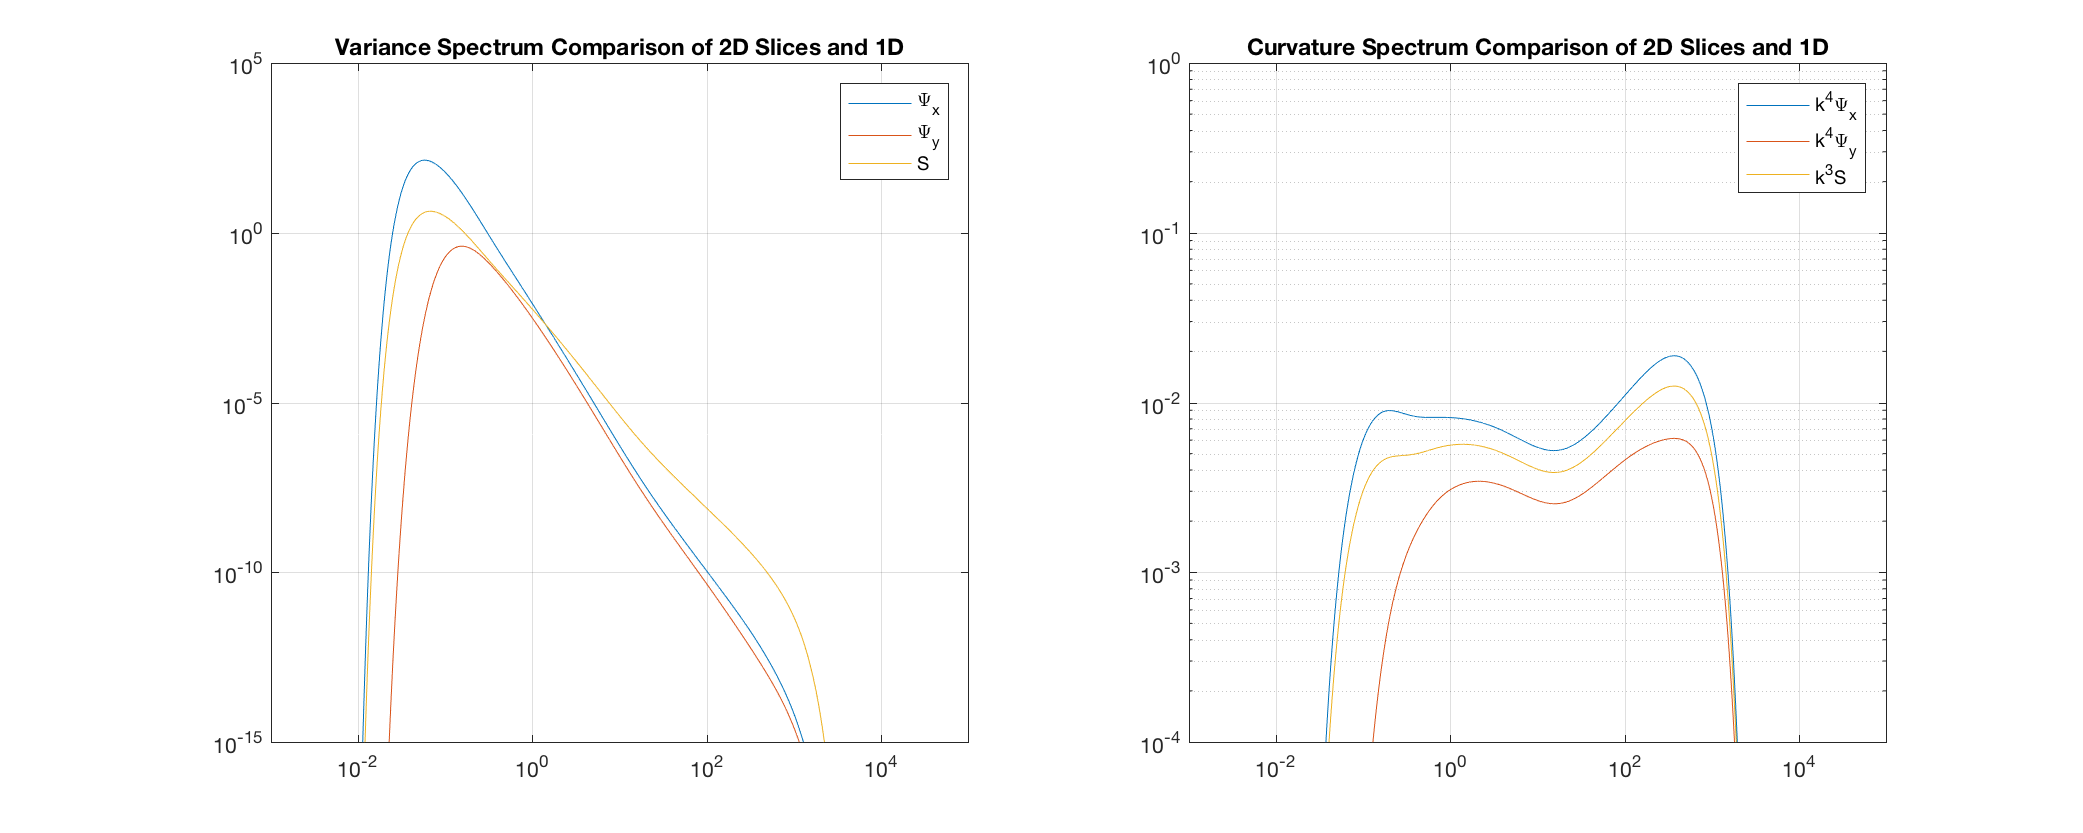
\includegraphics[width=6in]{../media/Ocean_Surface/elf_variance_curvature_spectrum_2D_slices.png}
  \end{center}
  \renewcommand{\baselinestretch}{1} \small\normalsize
  \begin{quote}
    \caption[Elfouhaily 2-D and 1D Variance and Curvature Power Spectra]{Elfouhaily 2-D and 1-D Variance and Curvature Power Spectra\label{os_fig:7bc}}
  \end{quote}
\end{figure}
\renewcommand{\baselinestretch}{2} \small\normalsize

Figure \ref{os_fig:7cc} shows the low frequency behavior of the 2-D variance power spectrum for $|k| \leq$ 2 rad/m.
\begin{figure}[H]
  \begin{center}
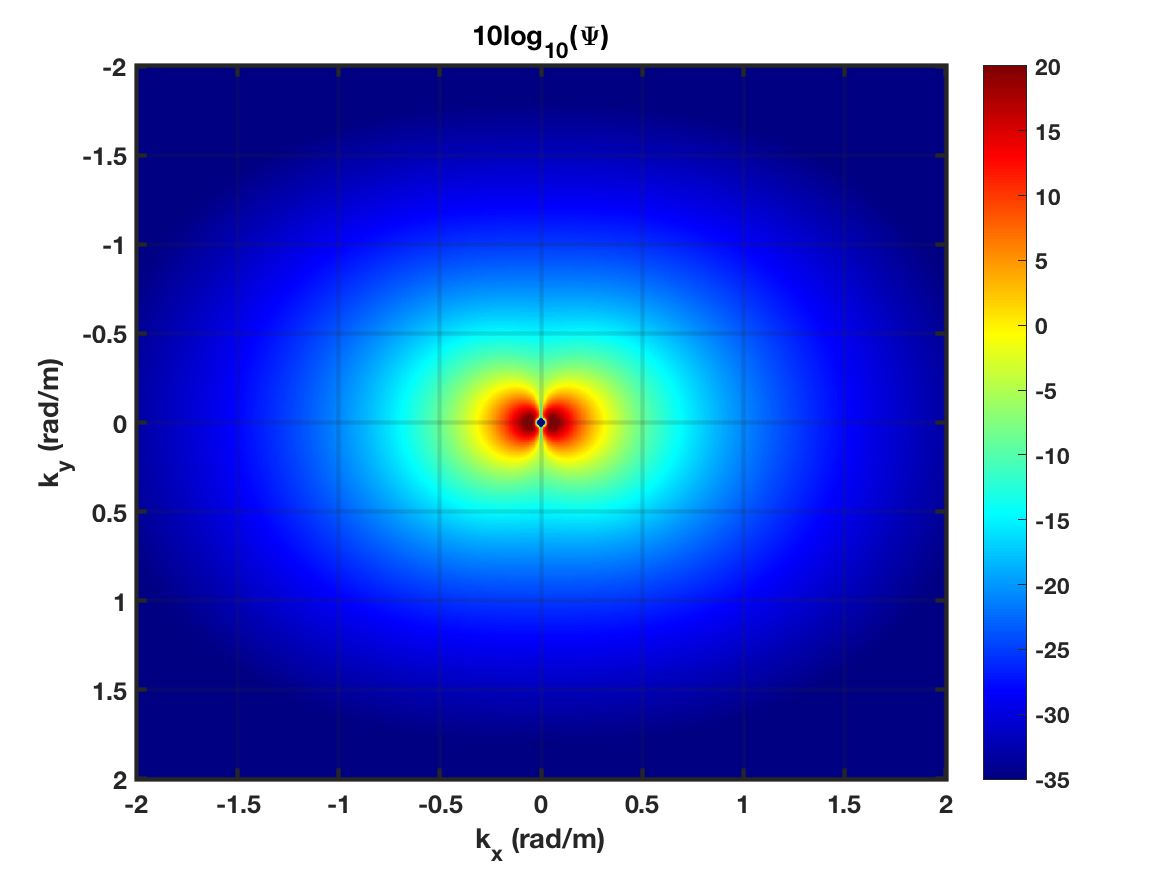
\includegraphics[width=4in]{../media/Ocean_Surface/elf_variance_spectrum_2D_zoom.png}
  \end{center}
  \renewcommand{\baselinestretch}{1} \small\normalsize
  \begin{quote}
    \caption[Elfouhaily 2-D Variance Power Spectrum]{Elfouhaily 2-D Variance Power Spectrum\label{os_fig:7cc}}
  \end{quote}
\end{figure}
\renewcommand{\baselinestretch}{2} \small\normalsize

\section{Sampling Constraints}\label{os_label:1d_sampling_constraints}
In order to generate a random sea surface, we need to establish the number of points to use ($N$) and the spatial domain length to cover ($L$). The spatial domain sampling inteval is given by $\Delta x = \frac{L}{N}$ and the frequency domain sampling interval is given by $\Delta k = \frac{2\pi}{L}$. 

\subsection{Spatial Domain Constraints}
The spatial domain length will have a lower bound driven by the frequency of the spectral peak. From the Nyquist theorem, the spatial sampling frequency must be less than or equal to 1/2 the spectral peak in order to recover that frequency. Because most of the energy is around the spectral peak, sampling at half the peak frequency is insufficient. A general rule of thumb is to use a factor of 1/10 to 1/20.

Figure \ref{os_fig:6ba} shows the sampled Elfouhaily variance power spectrum in linear units with $U_{10}$ = 10 m/s and $\Omega$ = 0.84.  The upper left hand plot shows the sampling when $\Delta k$ = $1/2 k_p$, the upper right hand plot shows the sampling when $\Delta k$ = $1/5 k_p$, the lower left hand plot shows the sampling when $\Delta k$ = $1/10 k_p$, and the upper right hand plot shows the sampling when $\Delta k$ = $1/20 k_p$. The peak power and 1/2 power points are identified by the horizontally dashed lines. We can see that for the case where $\Delta k$ = $1/2 k_p$, there are only 2 points sampled above half power in the spectrum. For the case where $\Delta k$ = $1/5 k_p$, there are 5 points sampled above half power. This is an improvement, but the spacing over the spectral peak is still coarse and the peak is not adequately sampled until $\Delta k \leq 1/10 k_p$
\begin{figure}[H]
  \begin{center}
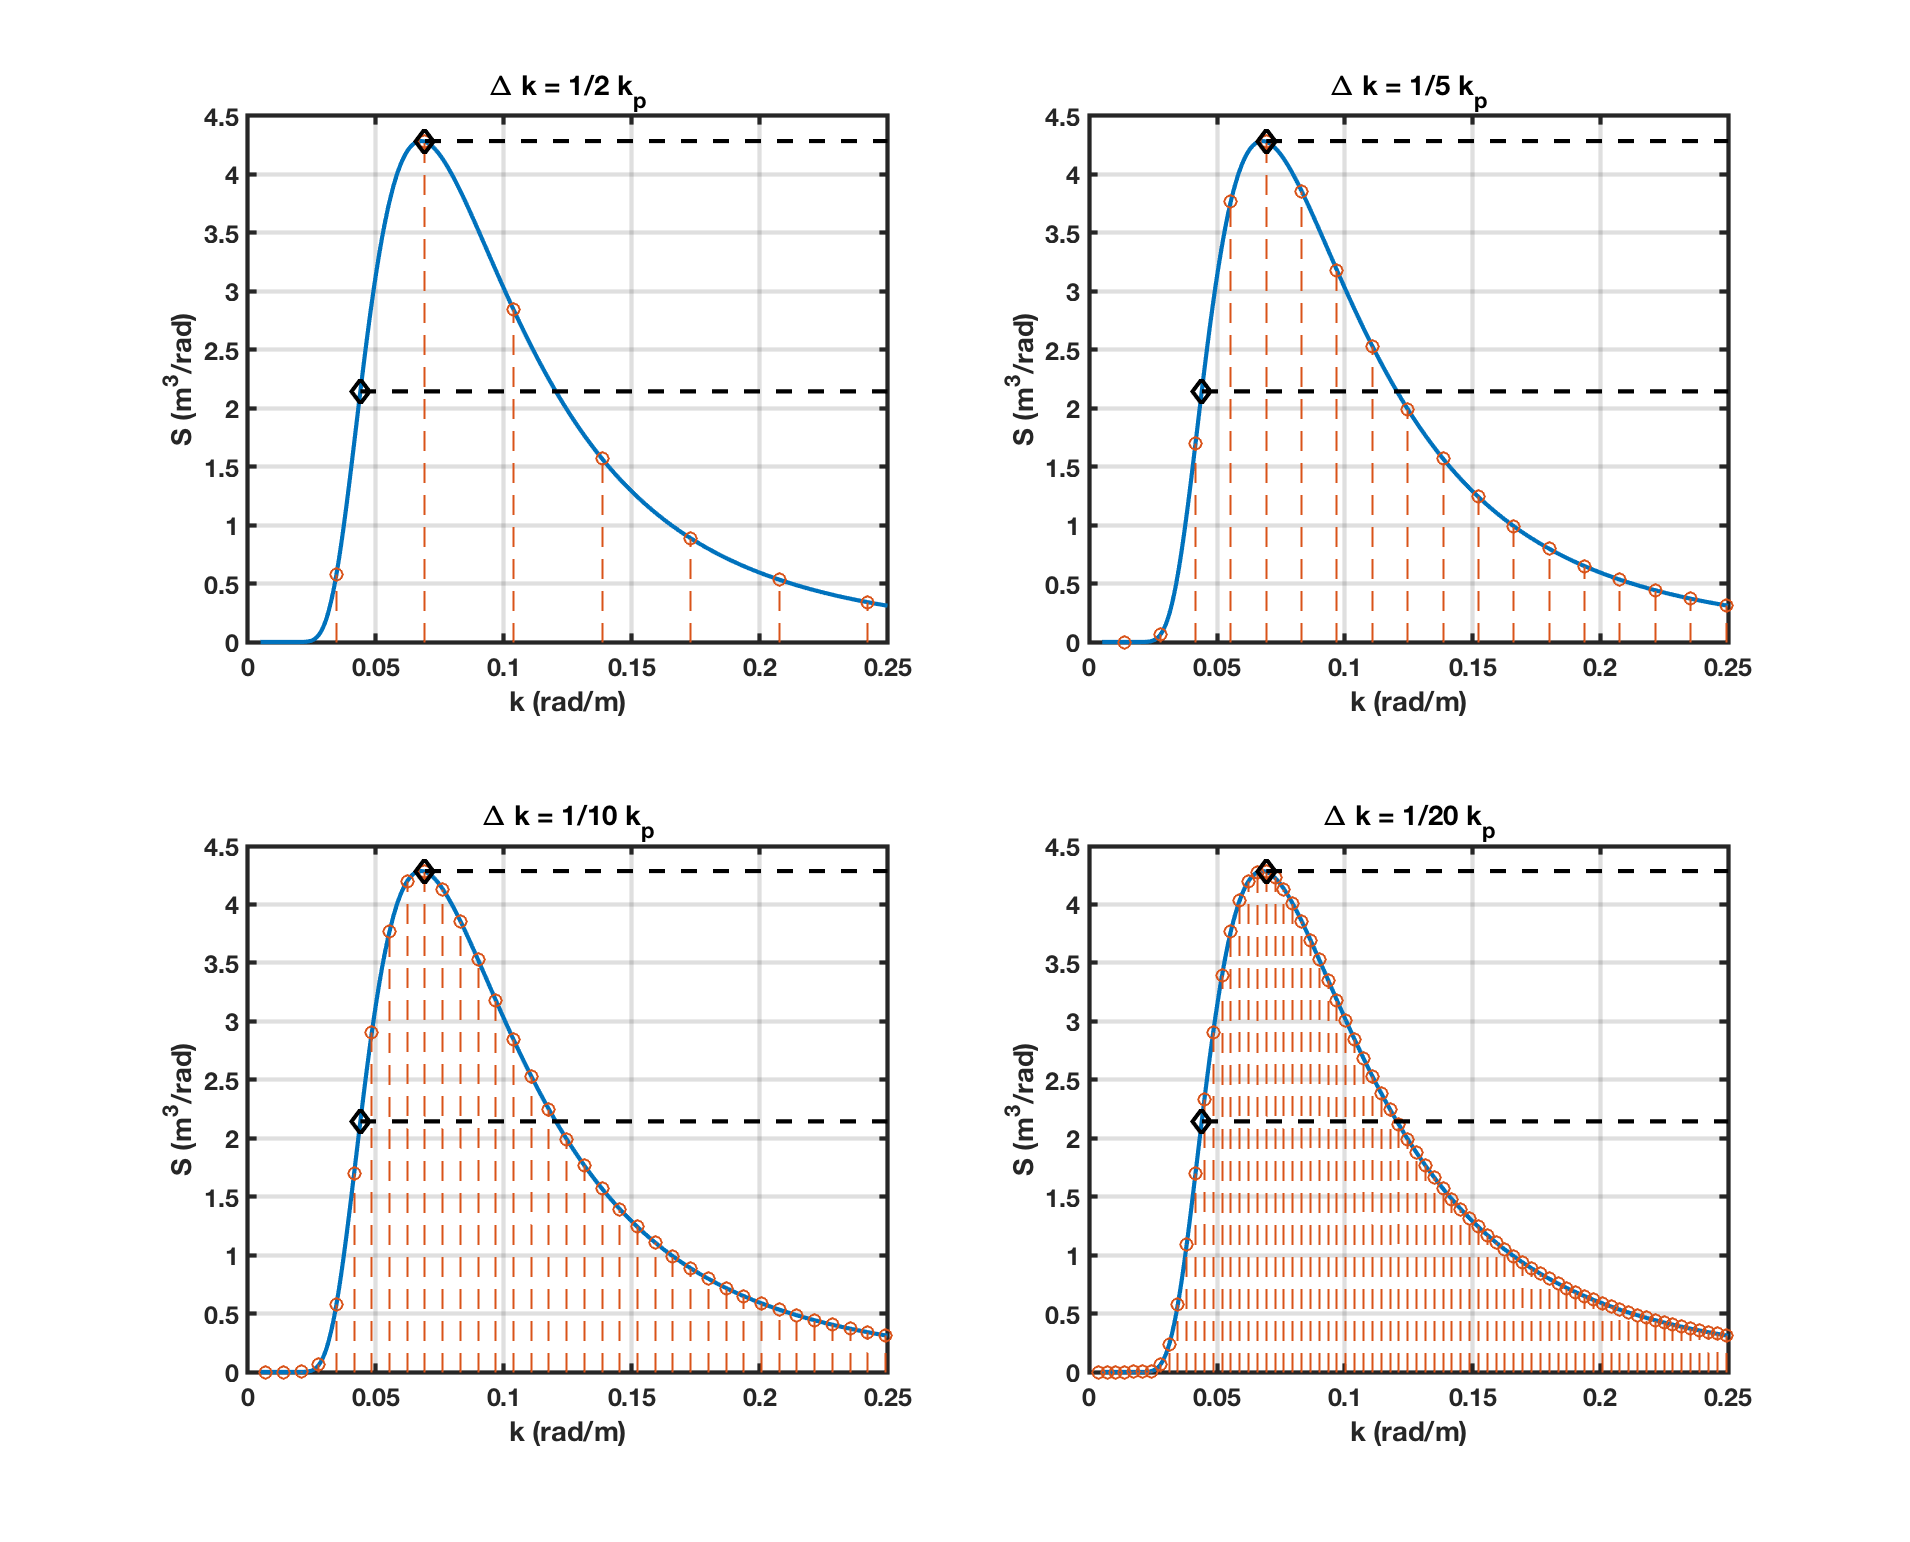
\includegraphics[width=6in]{../media/Ocean_Surface/spectral_peak_sampling.png}
  \end{center}
  \renewcommand{\baselinestretch}{1} \small\normalsize
  \begin{quote}
    \caption[Sampling Constraints for the Spectral Peak]{Sampling Constraints for the Spectral Peak\label{os_fig:6ba}}
  \end{quote}
\end{figure}
\renewcommand{\baselinestretch}{2} \small\normalsize

From Equation \ref{os_eq:3a}, we have $k_p = g\left(\frac{\Omega}{U_{10}}\right)^2$, so for Figure \ref{os_fig:6ba}, $k_p$ = 0.0692 rad/m. Using this equation, we can write the condition for the lower bound of $l$:
\begin{equation}
\label{os_eq:8o}
\boxed{L \geq \frac{20\pi}{g}\left(\frac{U_{10}}{\Omega} \right)^2}
\end{equation}

From Equation \ref{os_eq:8o}, the lower bound on $L$ will typically be between 1 km and 10 km. Generating a surface with a length smaller than this will result in inadequate sampling. The upper bound on $L$ will be limited either by the problem size we are covering or computational requirements due to the number of points.

\subsection{Constraints on Number of Points}
To determine $N$, we can look at sampling requirements for high spatial frequencies. From the Nyquist sampling theorem, the highest wave number that can be sampled is $k_{max} = \frac{N}{2}\Delta k = \frac{N\pi}{L}$ rad/m, which corresponds to a minimum wavelength of $\lambda_{min} = 2\Delta x = \frac{2L}{N}$ m.

Immediately, we can see that to sample the secondary peak at $k_m$, $\frac{N}{L}\pi > k_m$ or $N > \frac{k_m}{\pi}L$. Since $k_m = 370$ rad/m, we can round up to state that $N \geq 118L$ in this case. In other words, the number of points required to sample the secondary peak in the spectrum is 118 times more than the length of the spatial domain. For the 1-dimensional case, this is not too bad as the secondary peak for a 10 km length surface can be sampled with 1,180,000 points. In the 2-dimensional case, the number of points goes as $N^2$, and this will be a significant issue.

In general, we only need this many points when performing verification runs to demonstrate we are capable of modeling the entire spectrum correctly. The energy at the secondary peak is small compared to the energy at the primary peak. In many situations, we are not concerned with capturing the high spatial frequencies as much as we are with staying below a pre-defined maximum spatial step. This step is typically on the order of 0.1 m ($N = 10L$) to 0.5 m ($N = 2L$).

Figure \ref{os_fig:6aa} shows the impact on wavenumber sampling for various values of $N$ for $L$ = 1 km and $\Omega$ = 0.84. The upper left hand plot shows the case where $N = 2L$, the upper right hand plot shows the case where $N = 10L$, the lower left hand plot shows the case where $N = 118L$, and the lower right hand plot shows the case where $N = 500L$. Since $\Delta x = \frac{L}{N}$, these cases represent spatial resolutions of 1/2 m, 1/10 m, 1/118 m, and 1/500 m. 
\begin{figure}[H]
  \begin{center}
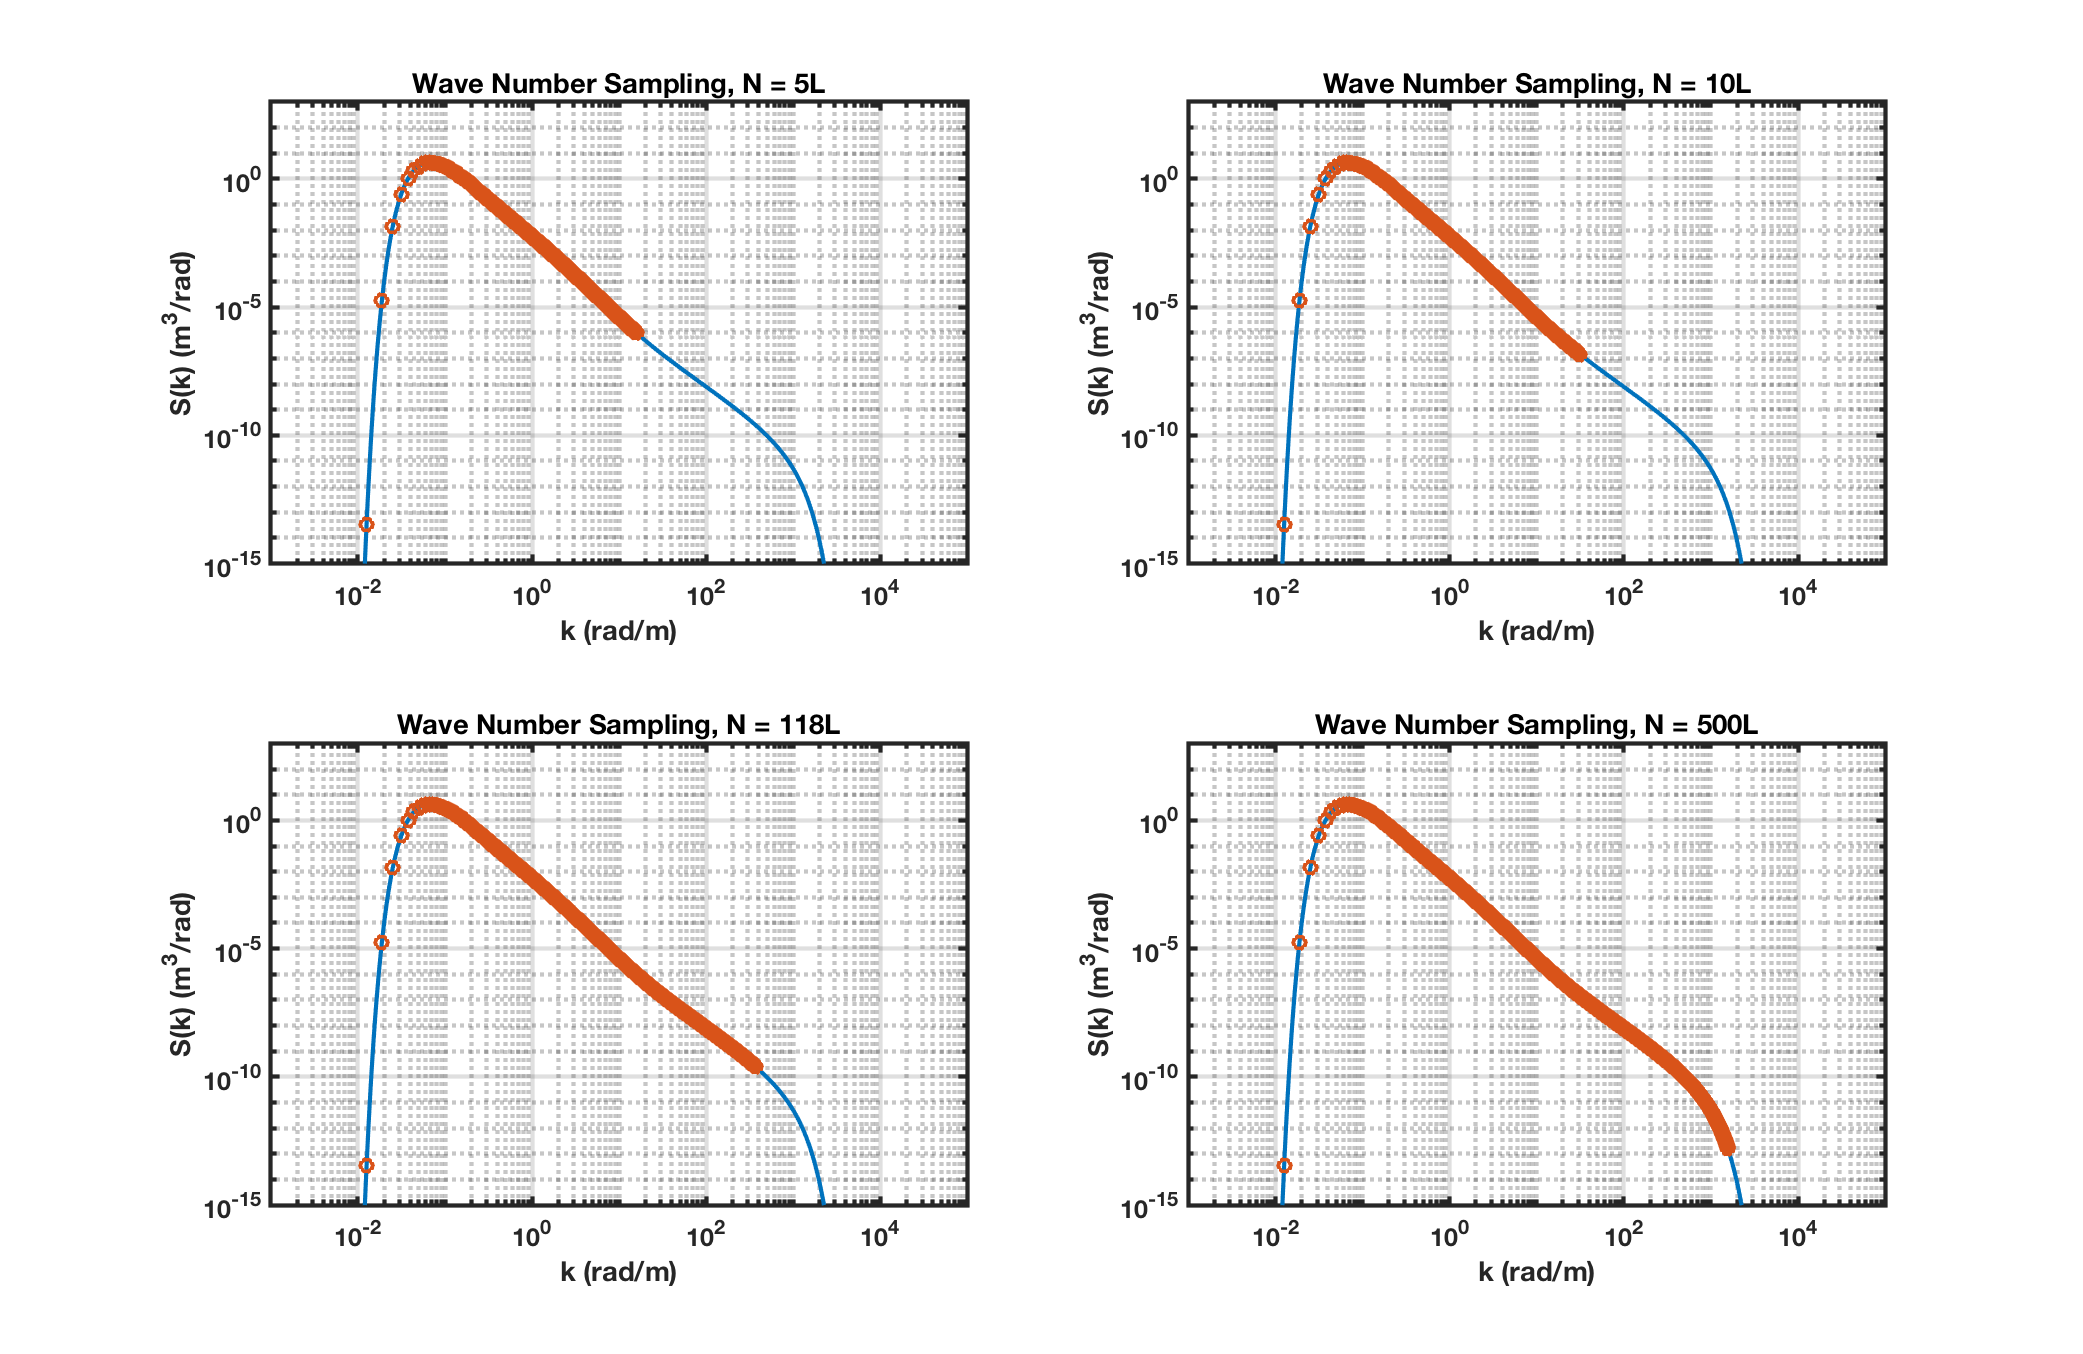
\includegraphics[width=6in]{../media/Ocean_Surface/sampling_coverage.png}
  \end{center}
  \renewcommand{\baselinestretch}{1} \small\normalsize
  \begin{quote}
    \caption[Wavenumber Sampling Coverage]{Wavenumber Sampling Coverage\label{os_fig:6aa}}
  \end{quote}
\end{figure}
\renewcommand{\baselinestretch}{2} \small\normalsize
Since $L$ is the same for each case, $\Delta k$ is also the same and we can see how increasing $N$ increases coverage of higher spatial frequencies.

As a final note for sampling constraints, we need to maintain integer indexing for digital implementation so $N$ must be an even integer to allow the element $N/2$ to be an integer as well. For the 1-dimensional case, we will define the range in $k$-space as running from $0$ to $\frac{N}{2}\Delta k$.

\section{Generation of Sea Surfaces in 1-Dimension}\label{os_sec:1d}
The general idea for generating sea surfaces is to use the power spectrum to create a realization of the sea surface in the frequency domain and then transform that to the spatial domain through an inverse Fourier transform. The 1-dimensional case is easiest to understand and implement and will be discussed first.

\subsection{Frequency Domain Representation}
The general idea is to use the power spectrum to create a realization of the sea surface in the frequency domain and then transform that to the spatial domain through an inverse Fourier transform. We will follow the procedure outlined in \cite{percival_spectra}, 
but we need to provide some additional scale factors to account for conservation of energy.

To handle discretization of the power spectrum, we use the fact that the amount of energy contained per unit interval is a constant, so that $S(k)dk = S(\omega) d\omega$. To normalize the spectrum to the specified wave number sampling interval, we simply need to multiply by $\Delta k$.

To generate the frequency domain representation ($V_j$), we will take a set of Gaussian distributed random variables that are scaled  by the square root of the power spectrum and arrange them so the sequence is Hermitian, $V(k) = V^*(-k)$. Because $N$ is even, as described in Section \ref{os_label:1d_sampling_constraints}, there are special cases to handle to ensure that the sequence is Hermitian. $V_j$ only contains a single element for $k = 0$ and $k = \frac{N}{2}\Delta k$ and must be purely real at both frequencies. If we take a pair of uncorrelated Gaussian distributed random variables of length $\frac{N}{2}$ ($w$ and $u$), we can generate $V_j$ as shown in Equation \ref{os_eq:8}.

\begin{equation}
  \label{os_eq:8}   
  V_j = \begin{cases}
    \sqrt{S_0\Delta k}w_0, & j = 0 \\
    \frac{1}{2}\sqrt{S_j\Delta k}\left[w_j + iu_j \right], & 1 \leq j < \frac{N}{2} \\
   \sqrt{S_{N/2}\Delta k}u_0 & j = \frac{N}{2} \\
    V_{N-j}^*, &  \frac{N}{2} < j \leq N-1 
  \end{cases} 
\end{equation}
The extra factor of $\frac{1}{2}$ in line 2 of Equation \ref{os_eq:8} comes from the fact that we have Hermitian symmetry and need to normalize both the expectations $\left<w_j + iu_j\right>$ and $\left<w_j - iu_j\right>$ to conserve energy.

The index ordering is assumed to have $k=0$ at the first element so that the sequence will wrap in frequency at $j = \frac{N}{2} + 1$. An example sequence for $N = 8$ is shown in Table \ref{os_tab:2a}.
\begin{table}[H]
  \begin{center}
      \renewcommand{\baselinestretch}{1} \small\normalsize
  \begin{quote}
    \caption[Example 1-Dimensional Frequency Domain Representation]{Example 1-Dimensional Frequency Domain Representation\label{os_tab:2a}}
  \end{quote}
  \begin{tabular} {| c | c | c |}
    \hline
  \bf{$j$} & \bf{$k_j$} & \bf{$V_j$} \\ \hline
  $0$ & $0$ & $\sqrt{S_{0} \Delta k}w_0$ \\ \hline
  $1$ & $\Delta k$ & $\frac{1}{2}\sqrt{S_1 \Delta k} \left(w_1 + iu_1 \right)$ \\ \hline
  $2$ & $2\Delta k$ & $\frac{1}{2}\sqrt{S_2\Delta k} \left(w_2 + iu_2 \right)$ \\ \hline
  $3$ & $3\Delta k$ & $\frac{1}{2}\sqrt{S_3 \Delta k} \left(w_3 + iu_3 \right)$ \\ \hline
  $4$ & $4\Delta k$ & $\sqrt{S_{4} \Delta k} u_0$ \\ \hline
  $5$ & $-3\Delta k$ & $\frac{1}{2}\sqrt{S_3 \Delta k} \left(w_3 - iu_3 \right)$ \\ \hline
  $6$ & $-2\Delta k$ & $\frac{1}{2}\sqrt{S_2 \Delta k} \left(w_2 - iu_2 \right)$  \\ \hline
  $7$ & $-\Delta k$ & $\frac{1}{2}\sqrt{S_1 \Delta k} \left(w_1 - iu_1 \right)$ \\ \hline
\end{tabular}
\end{center}
\end{table}
\renewcommand{\baselinestretch}{2} \small\normalsize

Figure \ref{os_fig:6ab} shows the Hermitian symmetry of the frequency domain representation graphically with $N$ = 8. The elements with frequencies $0$ and $4\Delta k$ (white boxes) have no symmetric frequencies and must be purely real. The other elements (colored boxes) do have symmetric frequencies and must be complex conjugates to each other (complex conjugate pairs are identified by the arrows).
\begin{figure}[H]
  \begin{center}
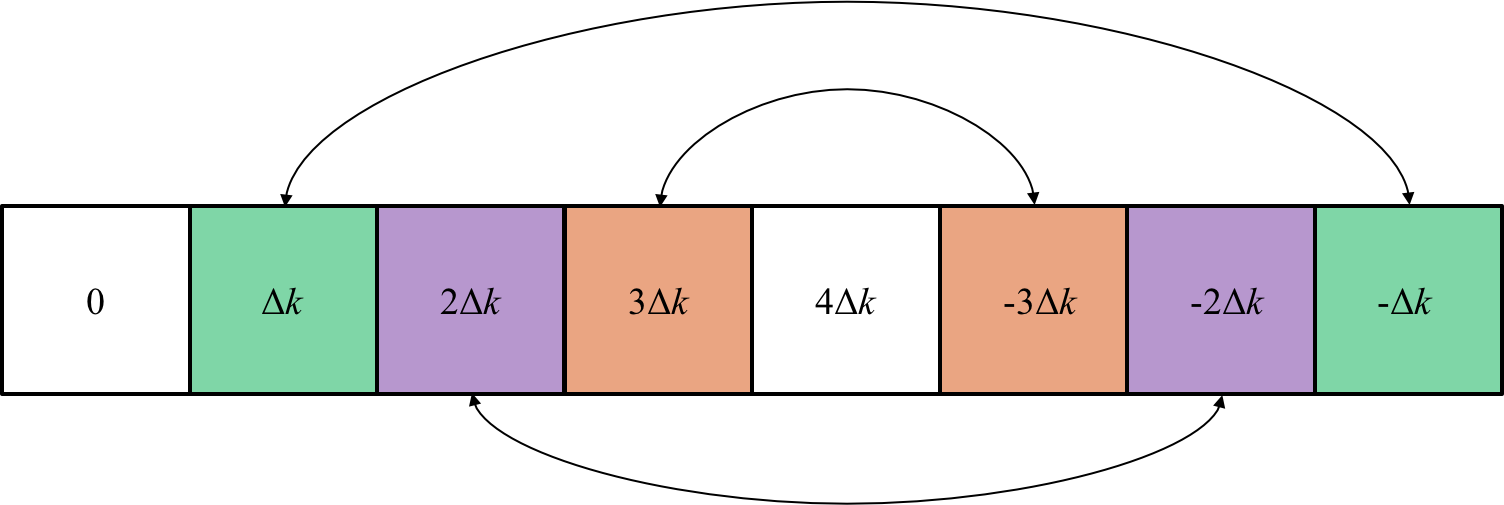
\includegraphics[width=5in]{../media/Ocean_Surface/1-d_hermitian_symmetry.png}
  \end{center}
  \renewcommand{\baselinestretch}{1} \small\normalsize
  \begin{quote}
    \caption[Hermitian Symmetry in 1-Dimension]{Hermitian Symmetry in 1-Dimension\label{os_fig:6ab}}
  \end{quote}
\end{figure}
\renewcommand{\baselinestretch}{2} \small\normalsize
Now that we have the coefficients in the frequency domain, we can generate the sea surface through the inverse Fourier transform as in Equation \ref{os_eq:9}. Because the sequence is Hermitian, the sea surface will be purely real.
\begin{equation}
  \label{os_eq:9}
  h(x) = \mathcal{F}^{-1}\left\{V(k) \right\}
  \end{equation}

\subsection{Example Realizations}
Figure \ref{os_fig:7a} shows an example realization for $U_{10}$ = 10 m/s and $L$ = 1 km. The right hand plot shows the generated sea surface for $N = 500L$ ($\Delta x$ = 1/500 m) and the bottom plot shows the same for $N=2L$ ($\Delta x$ = 1/2 m).
\begin{figure}[H]
  \begin{center}
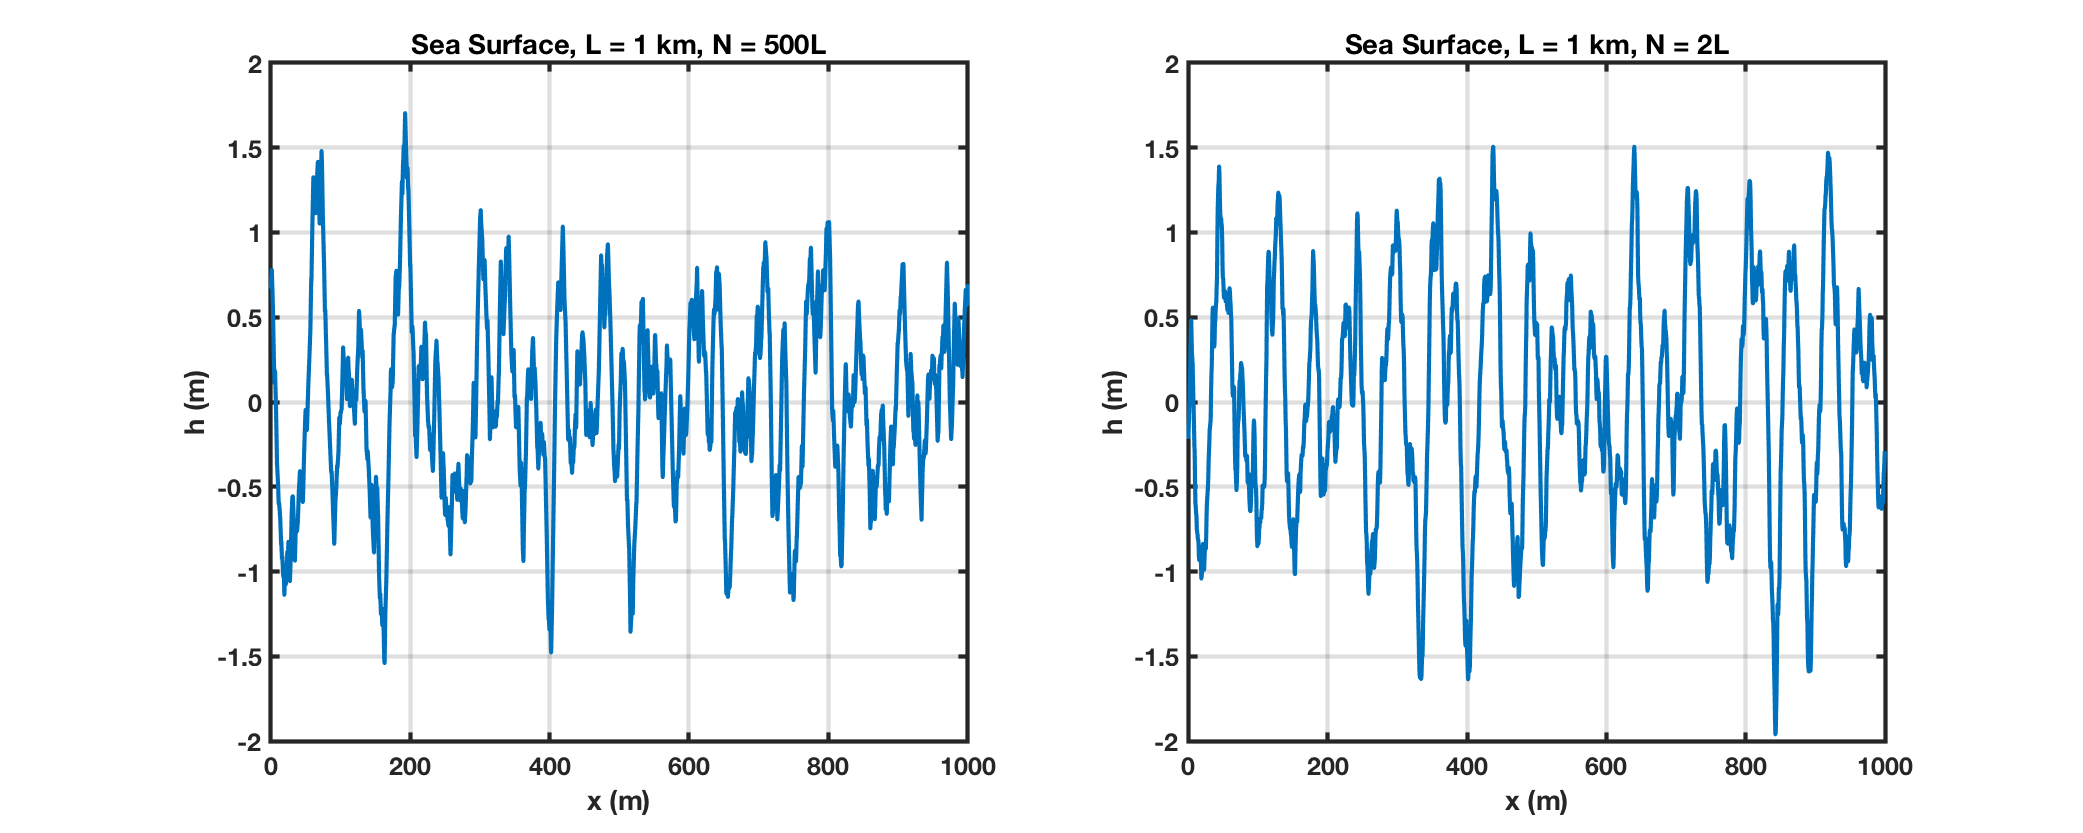
\includegraphics[width=6in]{../media/Ocean_Surface/sea_surface_1000.png}
  \end{center}
  \renewcommand{\baselinestretch}{1} \small\normalsize
  \begin{quote}
    \caption[Example Sea Surface Realization for 1 km Range]{Example Sea Surface Realization for 1 km Range\label{os_fig:7a}}
  \end{quote}
\end{figure}
\renewcommand{\baselinestretch}{2} \small\normalsize

Figure \ref{os_fig:7aa} sshows an example realization for $U_{10}$ = 10 m/s and $L$ = 10 km. The right hand plot shows the generated sea surface for $N = 500L$ ($\Delta x$ = 1/500 m) and the bottom plot shows the same for $N=2L$ ($\Delta x$ = 1/2 m).
\begin{figure}[H]
  \begin{center}
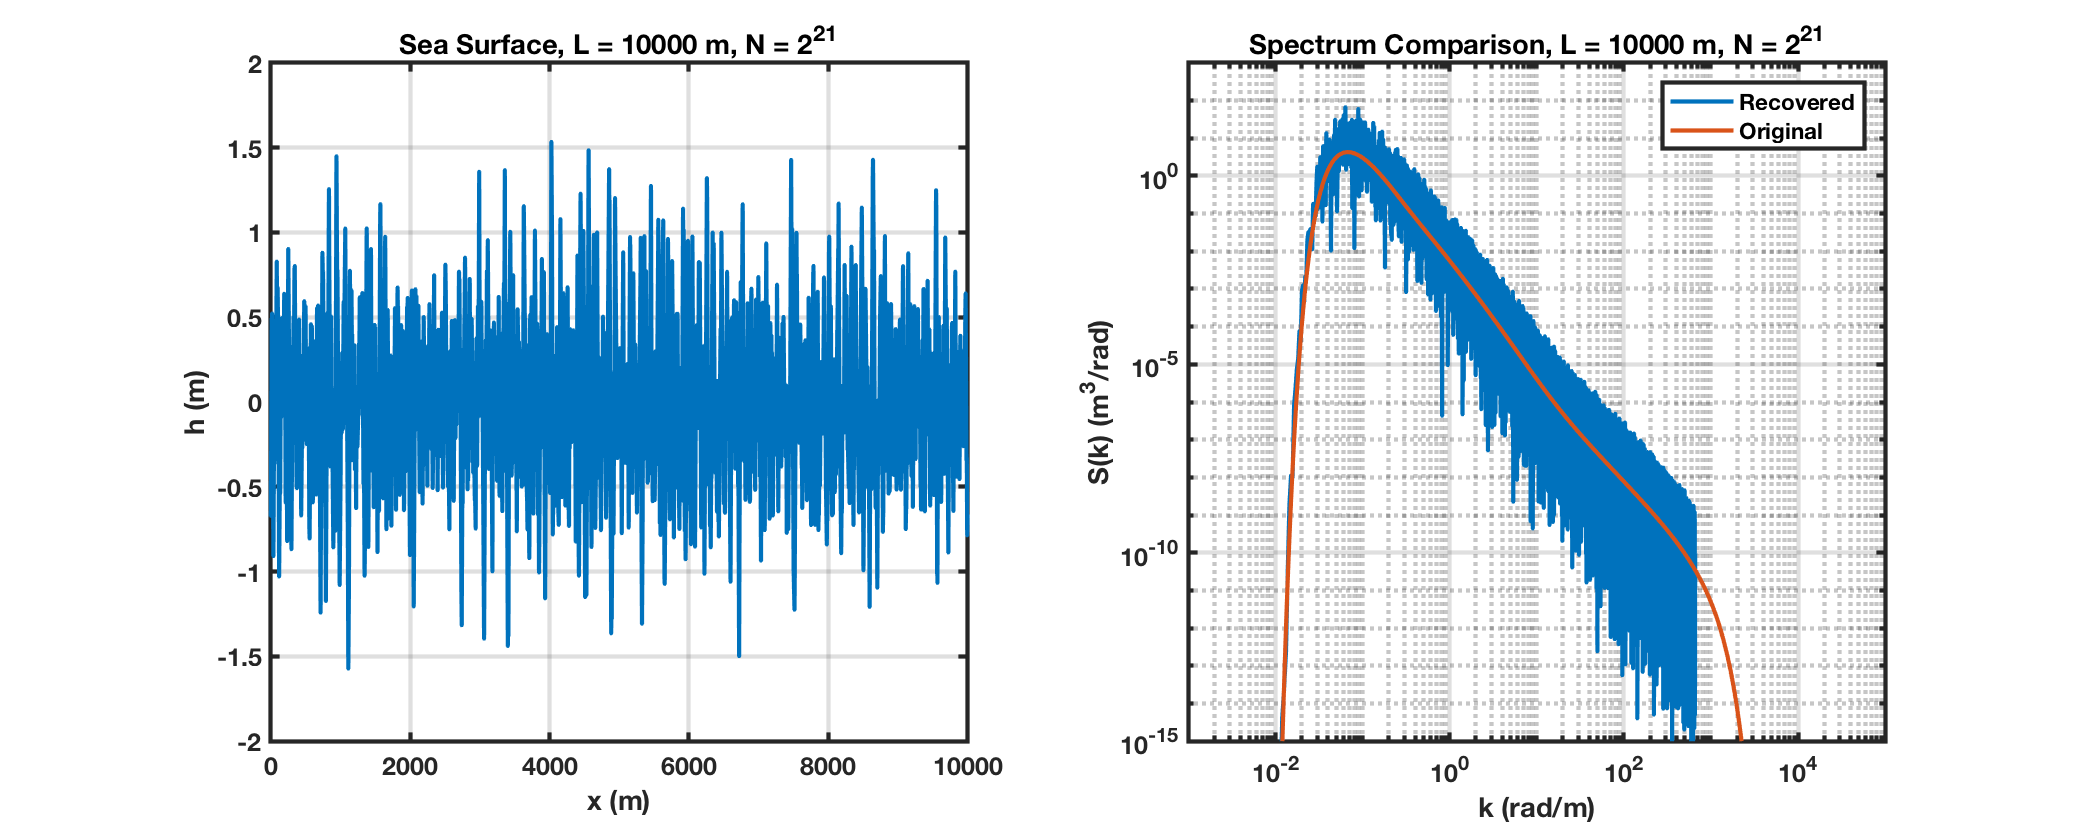
\includegraphics[width=6in]{../media/Ocean_Surface/sea_surface_10000.png}
  \end{center}
  \renewcommand{\baselinestretch}{1} \small\normalsize
  \begin{quote}
    \caption[Example Sea Surface Realization for 10 km Range]{Example Sea Surface Realization for 10 km Range\label{os_fig:7aa}}
  \end{quote}
\end{figure}
\renewcommand{\baselinestretch}{2} \small\normalsize

\section{Generation of Sea Surfaces in 2-Dimensions}
We will generally follow Section \ref{os_sec:1d} to generate 2-dimensional surfaces but we now have a wave vector $\mathbf{k} = k_x\hat{\mathbf{x}} + k_y\hat{\mathbf{y}}$ instead of a scalar wave number. In this case we will have matrices and the number of points will go as $N^2$. We still have the constraint that the frequency domain representation should exhibit Hermitian symmetry, so $V(n,m) = V^*(N-n,N-m)$. The special cases at the elements $k = 0$ and $k = \frac{N}{2}\Delta k$ now turn into special cases for the vectors $k_x = 0$, $k_x = \frac{N}{2}\Delta k$, $k_y = 0$, and $k_y = \frac{N}{2}\Delta k$. 

\subsection{Frequency Domain Representation}
The idea of Hermitian symmetry is less intuitive for 2-dimensions than 1-dimension. We should be careful to point out that the property of Hermitian symmetry does not imply that the matrix itself is Hermitian, as in general $V \neq V^H$. Figure \ref{os_fig:7dd} shows the symmetry properties for an $8 \times 8$ matrix ($N$ = 8) in terms of $(k_x, k_y)$ pairs. Here, the arrows identify the groupings that show symmetry. 
\begin{figure}[H]
  \begin{center}
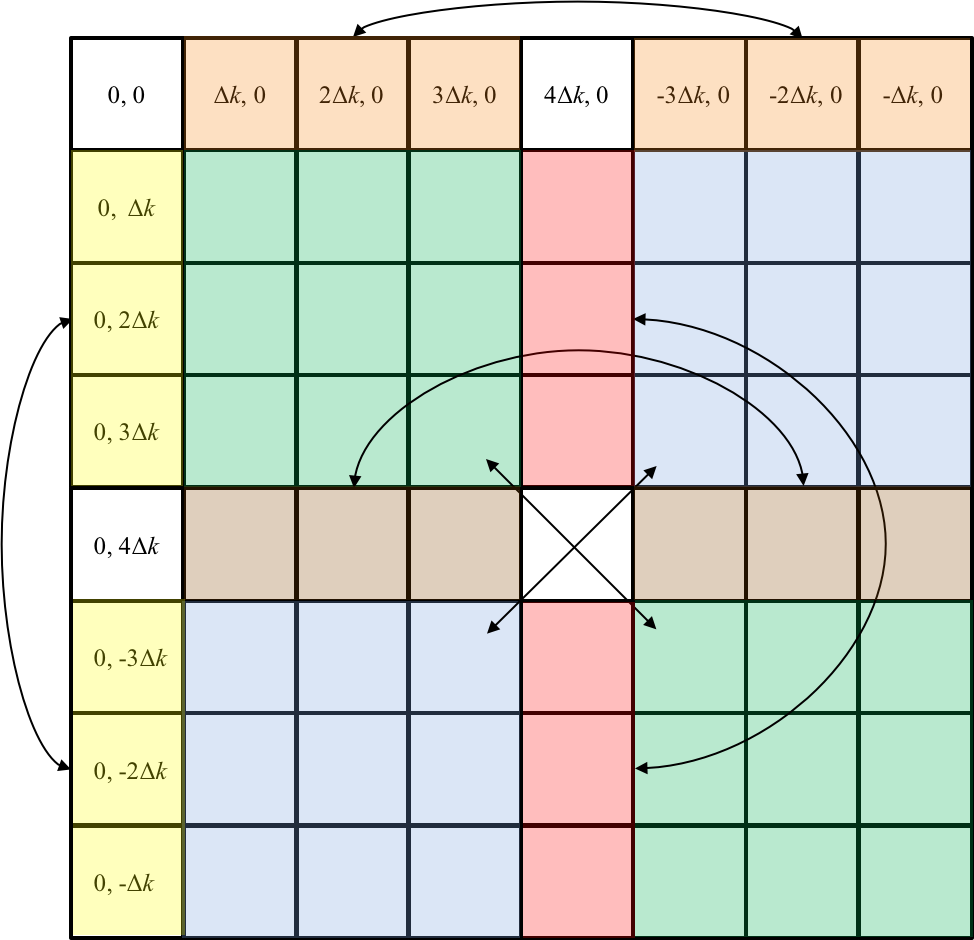
\includegraphics[width=4in]{../media/Ocean_Surface/2-d_hermitian_symmetry.png}
  \end{center}
  \renewcommand{\baselinestretch}{1} \small\normalsize
  \begin{quote}
    \caption[Hermitian Symmetry in 2-Dimensions]{Hermitian Symmetry in 2-Dimensions \label{os_fig:7dd}}
  \end{quote}
\end{figure}
\renewcommand{\baselinestretch}{2} \small\normalsize
The 4 white blocks at $(k_x=0, k_y=0)$, $(k_x=4\Delta k, k_y=0)$, $(k_x=0, k_y=4\Delta k)$, and $(k_x=4\Delta k, k_y=4\Delta k)$ have no symmetric frequencies and must be purely real. The 4 vectors where $k_x = 0$, $k_x = 4\Delta k$, $k_y = 0$, and $k_y = 4\Delta k$ are again special cases with no symmetric frequencies in the 2nd dimension. These cases can be treated independently as if they were 1-dimensional sequences. This leaves a set of 4 sub-matrices of size $\frac{N}{2} - 1 \times \frac{N}{2} - 1$. It is sufficient to compute 2 of the sub-matrices directly ($\mathbf{A}$ and $\mathbf{B}$) and then use the Hermitian symmetry property to generate the remaining 2 sub-matrices ($\mathbf{C}$ and $\mathbf{D}$).

The process to generate the frequency domain representation starts by using Equation \ref{os_eq:8} to cover the 4 special cases where $k_x = 0$, $k_x = \frac{N}{2}\Delta k$, $k_y = 0$, and $k_y = \frac{N}{2}\Delta k$. Each case will produce a sequence of length $N$, and should use independent sets of random variables $w$ and $u$ and the full 2-dimensional spectrum $\Psi$ instead of $S$. This is shown in Equation \ref{os_eq:9a} where $\alpha$ represents the spatial case being considered ($\alpha = 0$ or $\alpha = \frac{N}{2}$).

\begin{equation}
  \label{os_eq:9a}   
  V(\alpha,j) = \begin{cases}
    \sqrt{\Psi(\alpha,j)\Delta k^2}w(0), & j = 0 \\
    \frac{1}{2}\sqrt{\Psi(\alpha,j)\Delta k^2}\left[w(j) + iu(j) \right], & 1 \leq j < \frac{N}{2} \\
   \sqrt{\Psi(\alpha,N/2)\Delta k^2}u(0) & j = \frac{N}{2} \\
    V(\alpha,N-j)^*, &  \frac{N}{2} < j \leq N-1 
  \end{cases} 
\end{equation}

We can then generate 4 matrices of random variables ($W_1$, $W_2$, $U_1$, and $U_2$) with dimensions $\frac{N}{2} - 1 \times \frac{N}{2} - 1$ and compute $\mathbf{A}$ from Equation \ref{os_eq:10} and $\mathbf{B}$ from Equation \ref{os_eq:11}.

\begin{equation}
\label{os_eq:10}
\mathbf{A}(m,n) = \frac{1}{2}\sqrt{\Psi(m+1,n+1)\Delta k^2}\left[W_1(m,n) + iW_2(m,n) \right]
\end{equation}

\begin{equation}
\label{os_eq:11}
\mathbf{B}(m,n) = \frac{1}{2}\sqrt{\Psi(m+ 1,n+\frac{N}{2} +1)\Delta k^2}\left[W_1(m,n) + iW_2(m,n) \right]
\end{equation}

In these equations, the offsets in indexing $\Psi$ ensure that the correct spectral component is used. As with Equation \ref{os_eq:8}, we have an extra scale factor of $\frac{1}{2}$ to account for the additional expectations.

We can then compute $\mathbf{C}$ and $\mathbf{D}$ from symmetry:
\begin{equation}
\label{os_eq:12}
\begin{gathered}
\mathbf{C}(m,n) = \mathbf{A}^*\left(\frac{N}{2} - m, \frac{N}{2} - n \right) \\
\mathbf{D}(m,n) = \mathbf{B}^*\left(\frac{N}{2} - m, \frac{N}{2} - n \right) \\
\end{gathered}
\end{equation}

Once we have all the pieces, we can lay everything down in the appropriate location in $V$.

\subsection{Example Realizations}
Figure \ref{os_fig:8} shows a generated 2D sea surface with $L$ = 1 km and $U_{10}$ = 10 m/s. The right hand plot shows an image of the entire 1000 square meter surface and the left hand plot shows a 3D rendering of the 100 square meter patch outlined in the red box in the upper left hand corner of the right hand plot.
\begin{figure}[H]
  \begin{center}
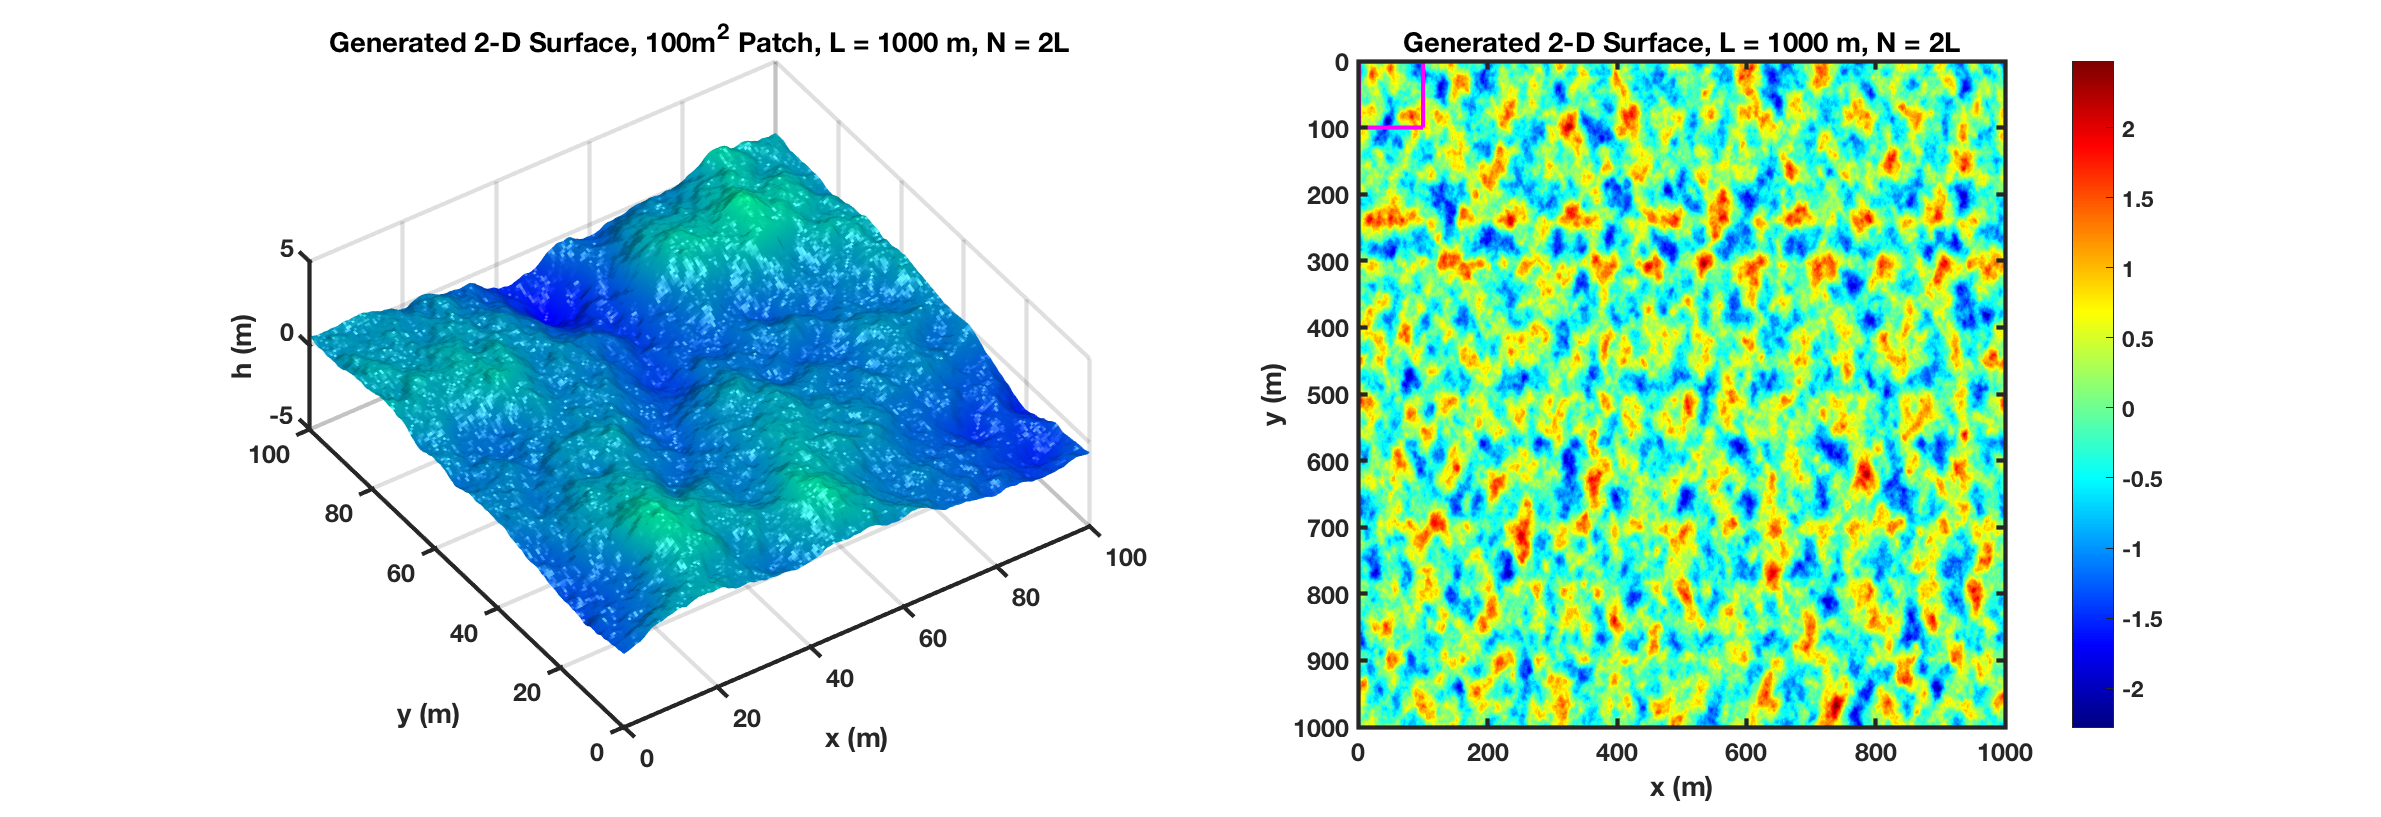
\includegraphics[width=6in]{../media/Ocean_Surface/sea_surface_2d_surf_1000.png}
  \end{center}
  \renewcommand{\baselinestretch}{1} \small\normalsize
  \begin{quote}
    \caption[Generated 2D Sea Surface, $L$ = 1 km]{Generated 2D Sea Surface, $L$ = 1 km \label{os_fig:8}}
  \end{quote}
\end{figure}
\renewcommand{\baselinestretch}{2} \small\normalsize

Figure \ref{os_fig:8a} shows the same thing as Figure \ref{os_fig:8} but with $N=10L$ instead of $N = 2L$.
\begin{figure}[H]
  \begin{center}
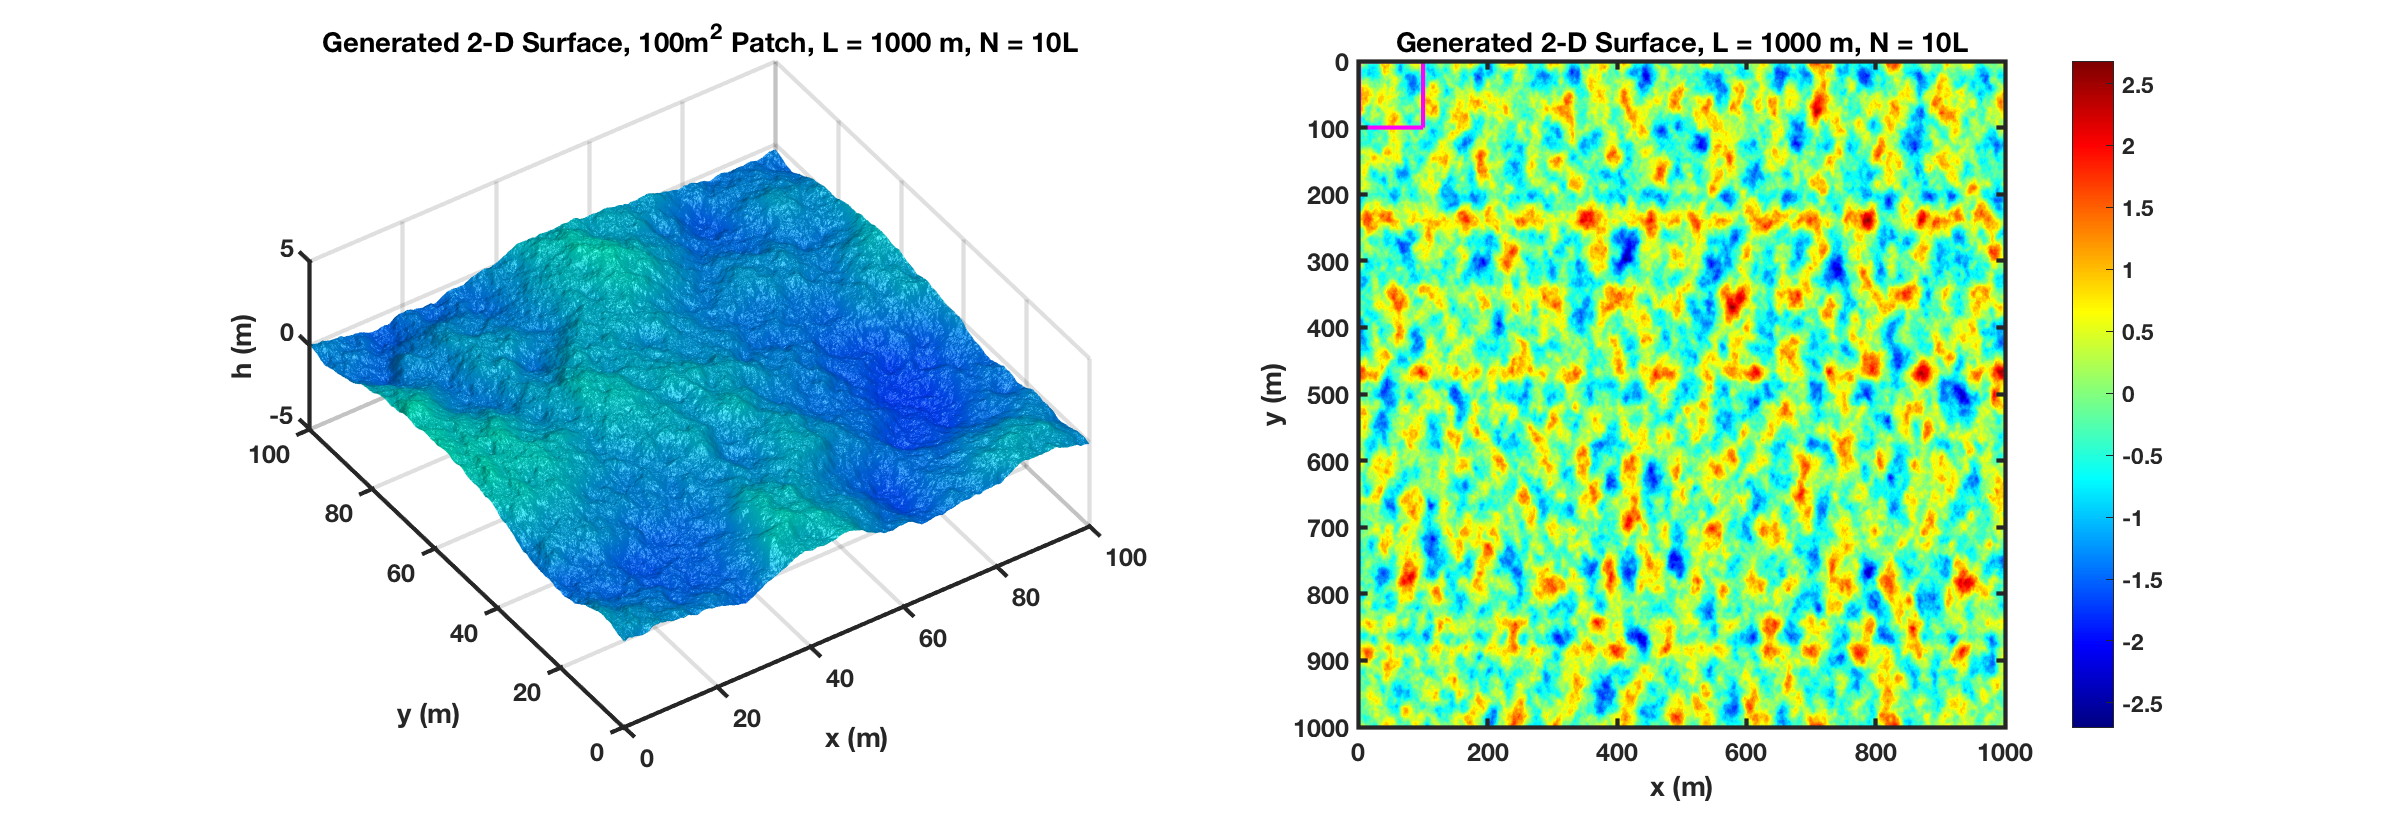
\includegraphics[width=6in]{../media/Ocean_Surface/sea_surface_2d_surf_1000_10.png}
  \end{center}
  \renewcommand{\baselinestretch}{1} \small\normalsize
  \begin{quote}
    \caption[Generated 2D Sea Surface, $L$ = 1 km, $N$ = 5$L$]{Generated 2D Sea Surface, $L$ = 1 km, $N$ = 5$L$ \label{os_fig:8a}}
  \end{quote}
\end{figure}
\renewcommand{\baselinestretch}{2} \small\normalsize

Figure \ref{os_fig:11} shows the generated sea surface for $L$ = 5 km, $N$= $2L$, and $U_{10}$ = 10 m/s. Again, the right hand plot shows an image of a 1000 square meter section of the surface and the left hand plot shows a 3D rendering of the 100 square meter patch outlined in the red box in the upper left hand corner of the right hand plot.
\begin{figure}[H]
  \begin{center}
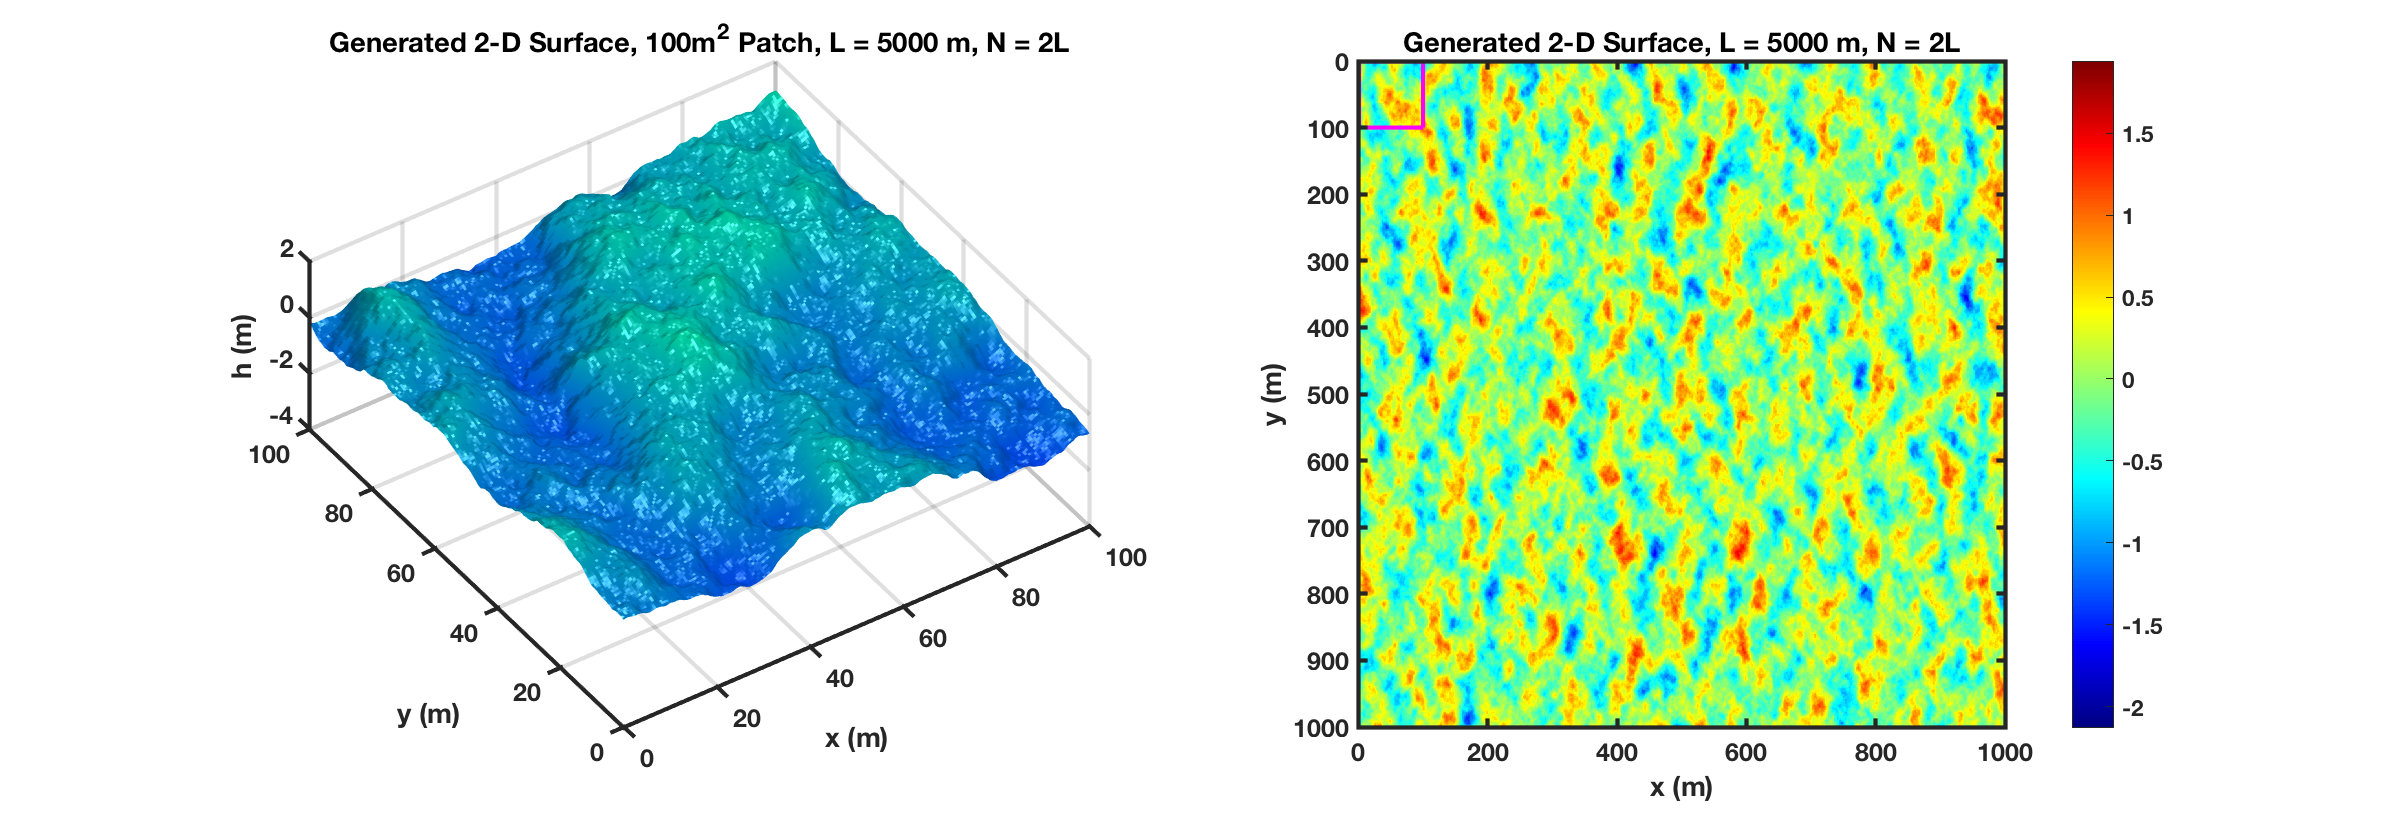
\includegraphics[width=6in]{../media/Ocean_Surface/sea_surface_2d_surf_5000.png}
  \end{center}
  \renewcommand{\baselinestretch}{1} \small\normalsize
  \begin{quote}
    \caption[Generated 2D Sea Surface, $L$ = 5 km]{Generated 2D Sea Surface, $L$ = 5 km \label{os_fig:11}}
  \end{quote}
\end{figure}
\renewcommand{\baselinestretch}{2} \small\normalsize

Figure \ref{os_fig:12} shows the generated sea surface for $L$ = 7.5 km , $N$ = $2L$, and $U_{10}$ = 10 m/s. Again, the right hand plot shows an image of a 1000 square meter section of the surface and the left hand plot shows a 3D rendering of the 100 square meter patch outlined in the red box in the upper left hand corner of the right hand plot.
\begin{figure}[H]
  \begin{center}
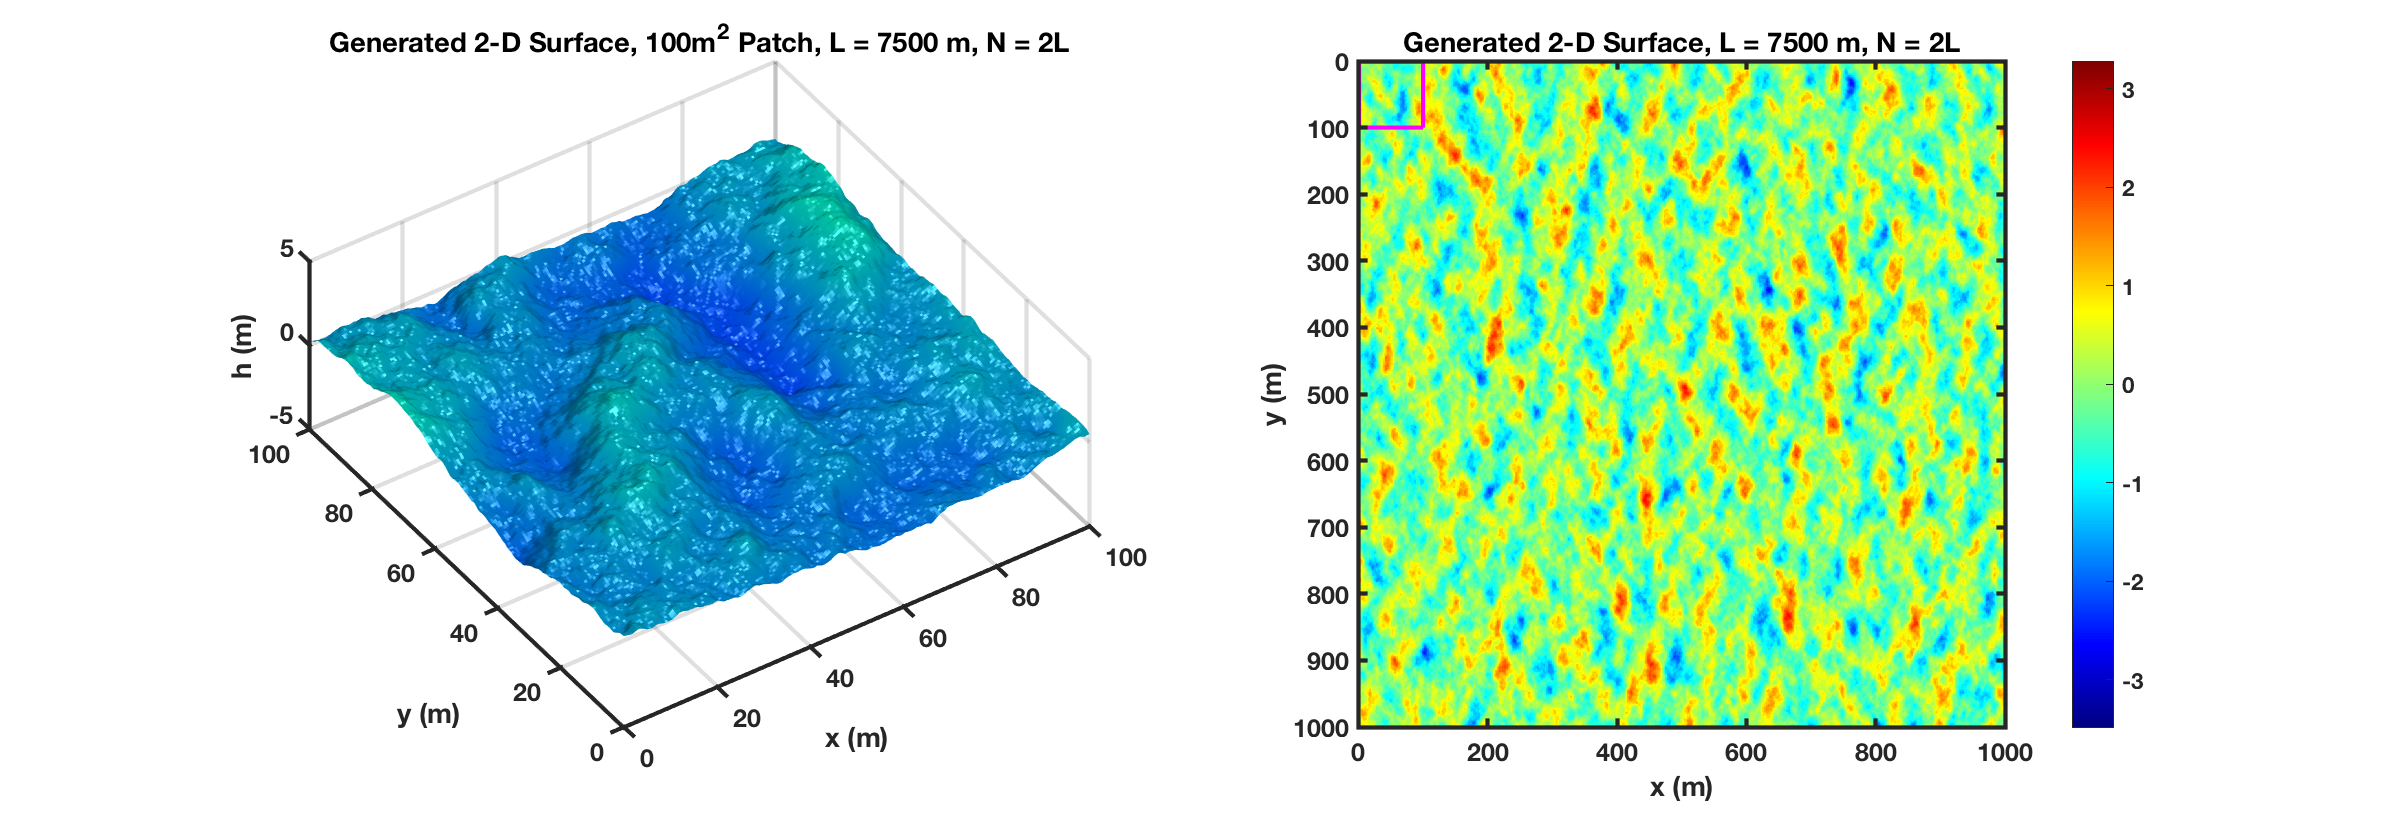
\includegraphics[width=6in]{../media/Ocean_Surface/sea_surface_2d_surf_7500.png}
  \end{center}
  \renewcommand{\baselinestretch}{1} \small\normalsize
  \begin{quote}
    \caption[Generated 2D Sea Surface, $L$ = 7.5 km]{Generated 2D Sea Surface, $L$ = 7.5 km \label{os_fig:12}}
  \end{quote}
\end{figure}
\renewcommand{\baselinestretch}{2} \small\normalsize

\section{Verification}
Verification testing is important to ensure that the computed sea surfaces have the appropriate statistics and that conservation of energy is maintained.

\subsection{Verification Process}
The verification process involves first generating a series of realizations to compare ensemble statistics. The overall wave height is compared against Table \ref{os_tab:0} and $\sigma_h$ is compared to Table 6.3 in the Tropospheric Electromagnetic Parabolic Equation Routine (TEMPER) user guide \cite{temper_guide}. The Ocean Surface Generator (OSG) mode added in TEMPER v3.2 internally uses the 1-dimensional Elfouhaily spectrum to generate random sea surface realizations and provides tables of ensemble statistics for comparison \cite{temper_guide}. 

The next step is to recover the power spectrum from the sea surface and compare it to the original power spectrum. Since we are operating in $k$-space and most computational FFT routines work in frequency space ($f_x$), we need to scale the results by $1/2\pi$. In the 2-D case, the full 2-D spectrum is estimated from the generated surface and then slices are taken to compare to slices from the original 2-D spectrum. 

\subsection{1-D Testing}
\subsubsection{Ensemble Statistics}
Figure \ref{os_fig:7fff} shows the RMS wave height vs. wind speed and is consistent with Table 6.3 and Figure 6.6 in \cite{temper_guide}.
\begin{figure}[H]
  \begin{center}
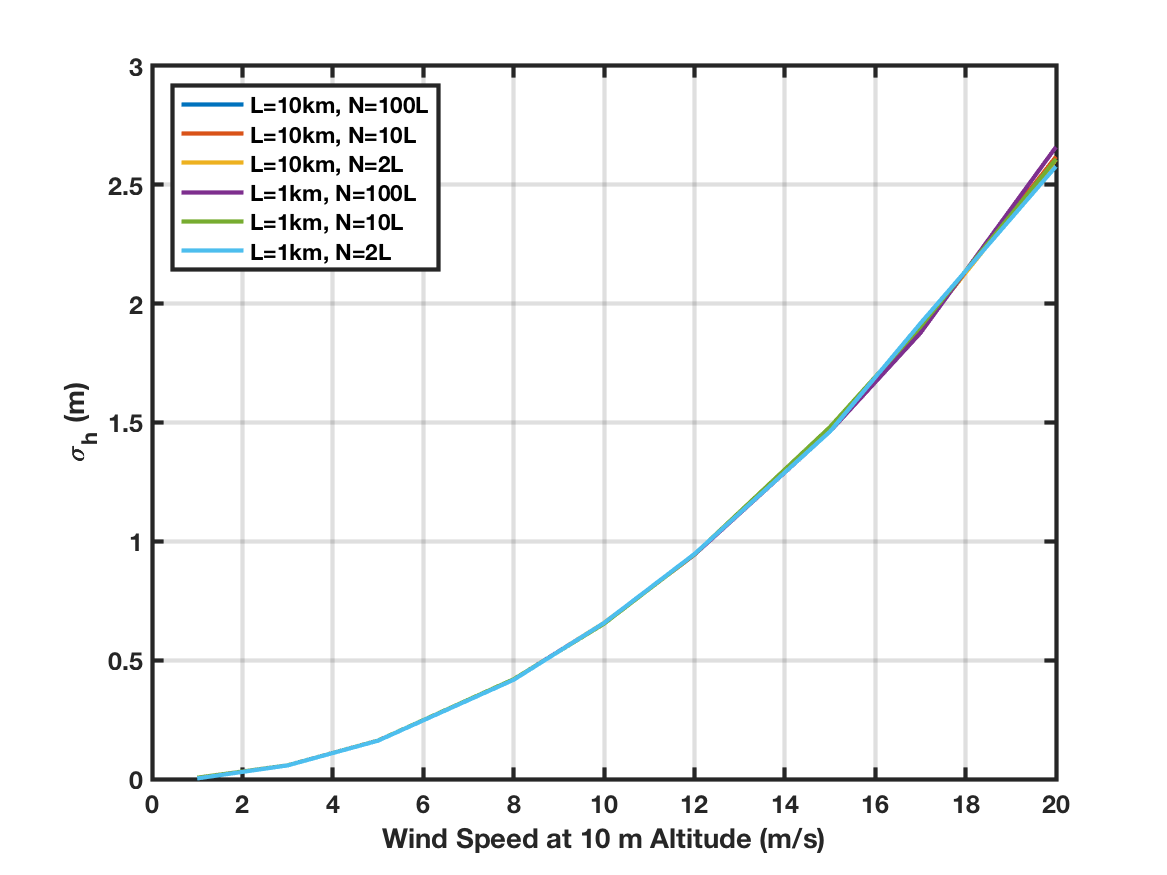
\includegraphics[width=6in]{../media/Ocean_Surface/1d_ensemble_rms.png}
  \end{center}
  \renewcommand{\baselinestretch}{1} \small\normalsize
  \begin{quote}
    \caption[$\sigma_h$ vs. Wind Speed for 1-Dimensional Sea Surface]{$\sigma_h$ vs. Wind Speed for 1-Dimensional Sea Surface\label{os_fig:7fff}}
  \end{quote}
\end{figure}
\renewcommand{\baselinestretch}{2} \small\normalsize
This figure shows the ensemble averages of 100 realizations for 6 different sampling conditions at various wind speeds. The conditions were set to $N$ = 2$L$, $N$ = 10$L$, and $N$ = 100$L$ for $L$ = 1 km and $L$ = 10 km. There is little difference in the RMS wave heights of any of the settings expect at high wind speeds. Because the wind speed shifts the spectral peak, the $L$ = 1 km cases are no longer adequately sampling the spectral peak at high wind speeds.

\subsubsection{Power Spectrum Recovery}
Figure \ref{os_fig:7bbb} shows the case for $U_{10}$ = 10 m/s and $L$ = 1 km. The left hand plot shows a comparison of the original spectrum to the recovered spectrum for $N = 500L$ ($\Delta x$ = 1/500 m) and the right hand plot shows the same for $N=2L$ ($\Delta x$ = 1/2 m).
\begin{figure}[H]
  \begin{center}
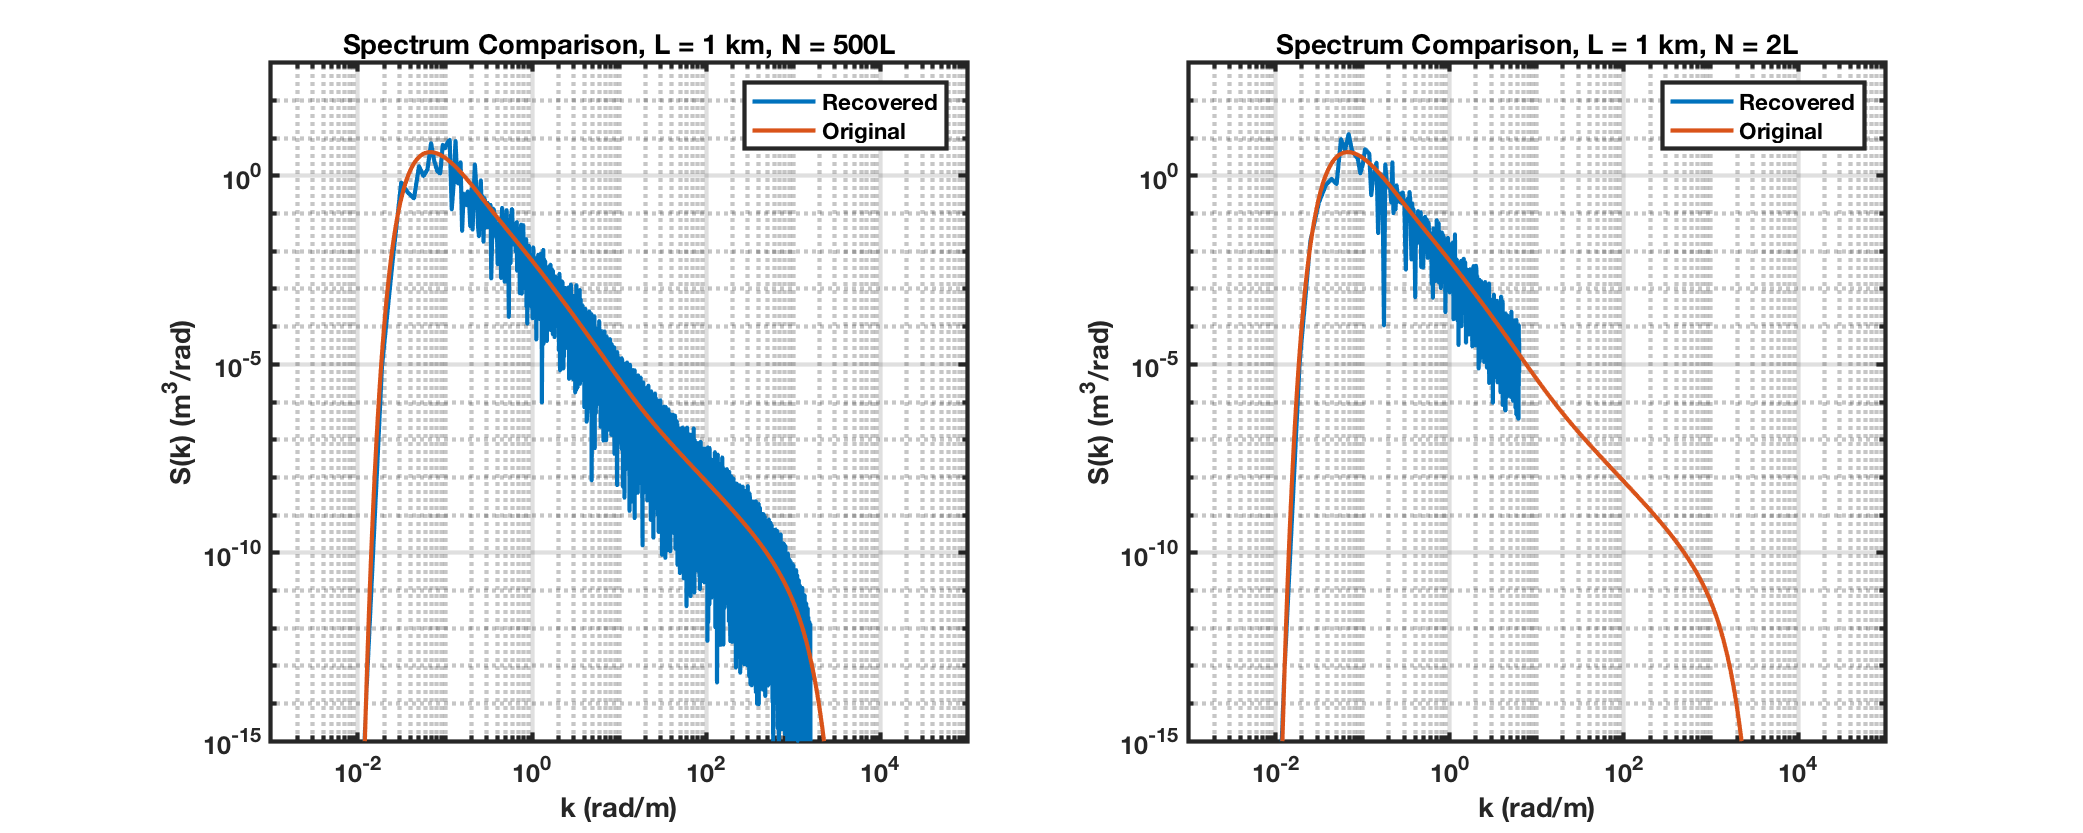
\includegraphics[width=6in]{../media/Ocean_Surface/sea_surface_spectra_1000.png}
  \end{center}
  \renewcommand{\baselinestretch}{1} \small\normalsize
  \begin{quote}
    \caption[Example Sea Surface Realization for 1 km Range]{Example Sea Surface Realization for 1 km Range\label{os_fig:7bbb}}
  \end{quote}
\end{figure}
\renewcommand{\baselinestretch}{2} \small\normalsize

Figure \ref{os_fig:7aaa} shows the case for $U_{10}$ = 10 m/s and $L$ = 10 km. The left hand plot shows a comparison of the original spectrum to the recovered spectrum for $N = 500L$ ($\Delta x$ = 1/500 m) and the right hand plot shows the same for $N=2L$ ($\Delta x$ = 1/2 m).
\begin{figure}[H]
  \begin{center}
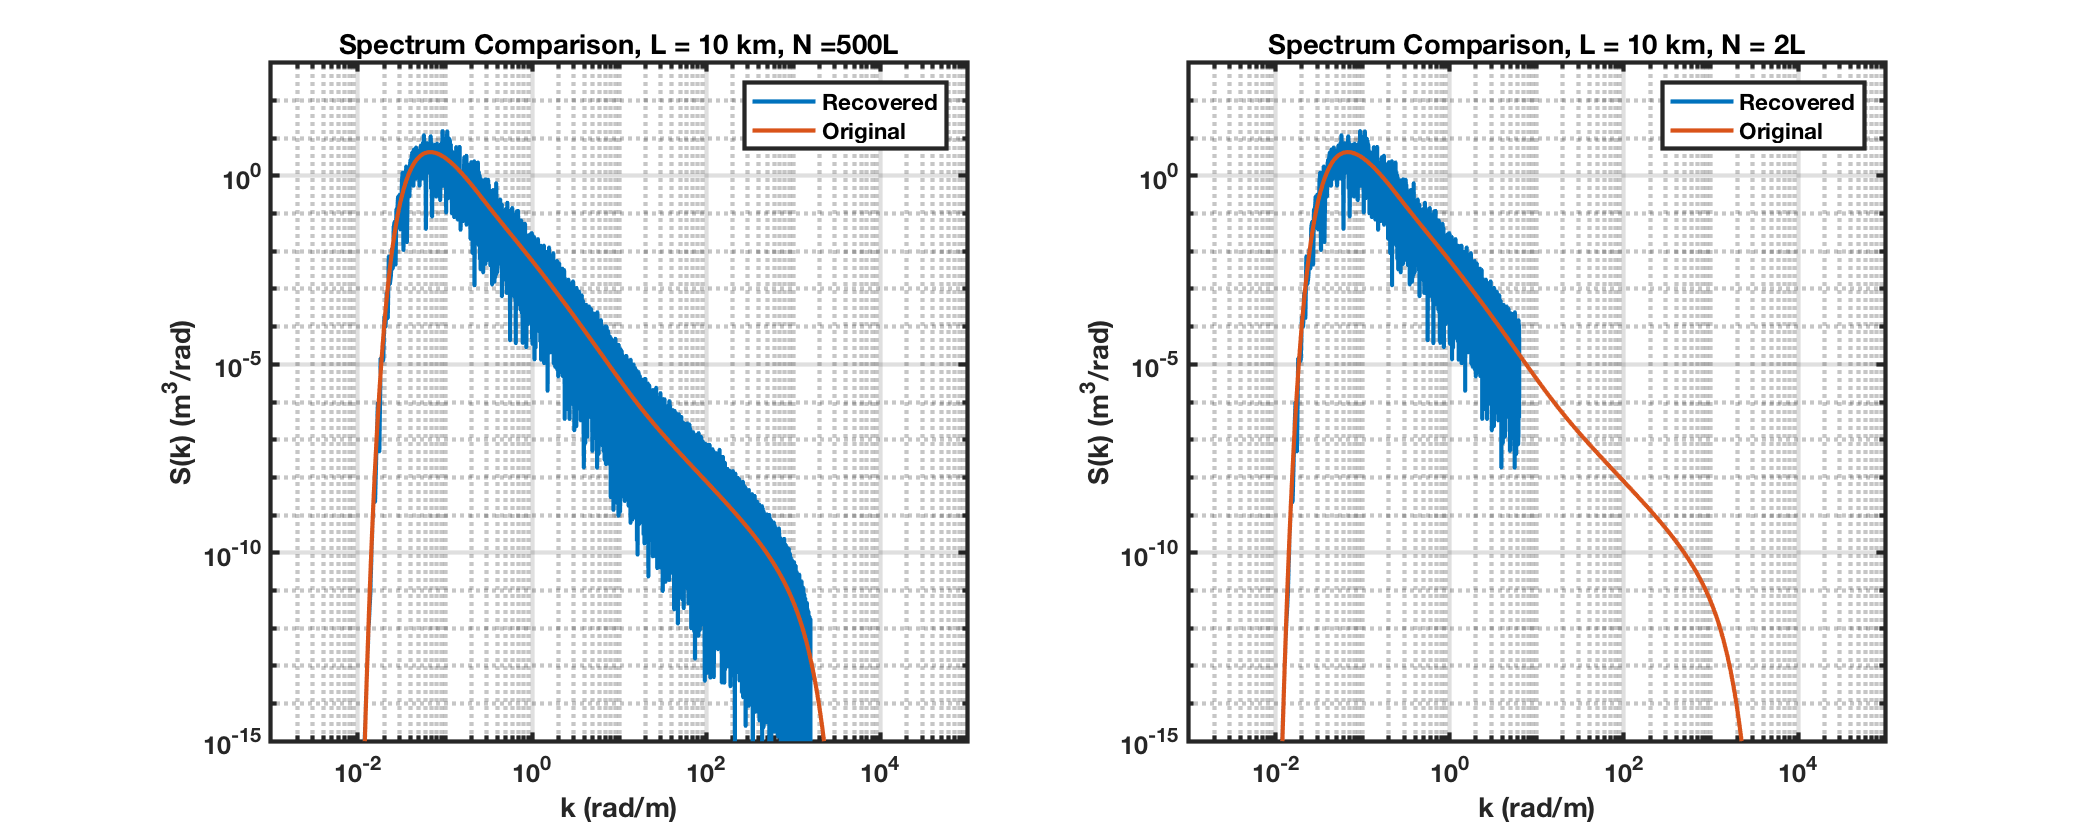
\includegraphics[width=6in]{../media/Ocean_Surface/sea_surface_spectra_10000.png}
  \end{center}
  \renewcommand{\baselinestretch}{1} \small\normalsize
  \begin{quote}
    \caption[Example Sea Surface Realization for 10 km Range]{Example Sea Surface Realization for 10 km Range\label{os_fig:7aaa}}
  \end{quote}
\end{figure}
\renewcommand{\baselinestretch}{2} \small\normalsize

\subsection{2-D Testing}
Testing in 2-dimensions is not as straightforward as in 1-dimension. The spectrum differs along the $x$ direction from the $y$ direction, so the statistics will be dependent on the direction.

\subsubsection{Ensemble Statistics}
TBD

\subsubsection{Power Spectrum Recovery}
For the $L$ = 1 km, $N$ = $2L$, and $U_{10}$ = 10 m/s case, Figure \ref{os_fig:10} shows slices along the $N/2$ element in both the $x$ and $y$ planes on the left hand side and a comparison of the spectral slices in the 2-D Elfouhaily spectrum on the right hand side. 
\begin{figure}[H]
  \begin{center}
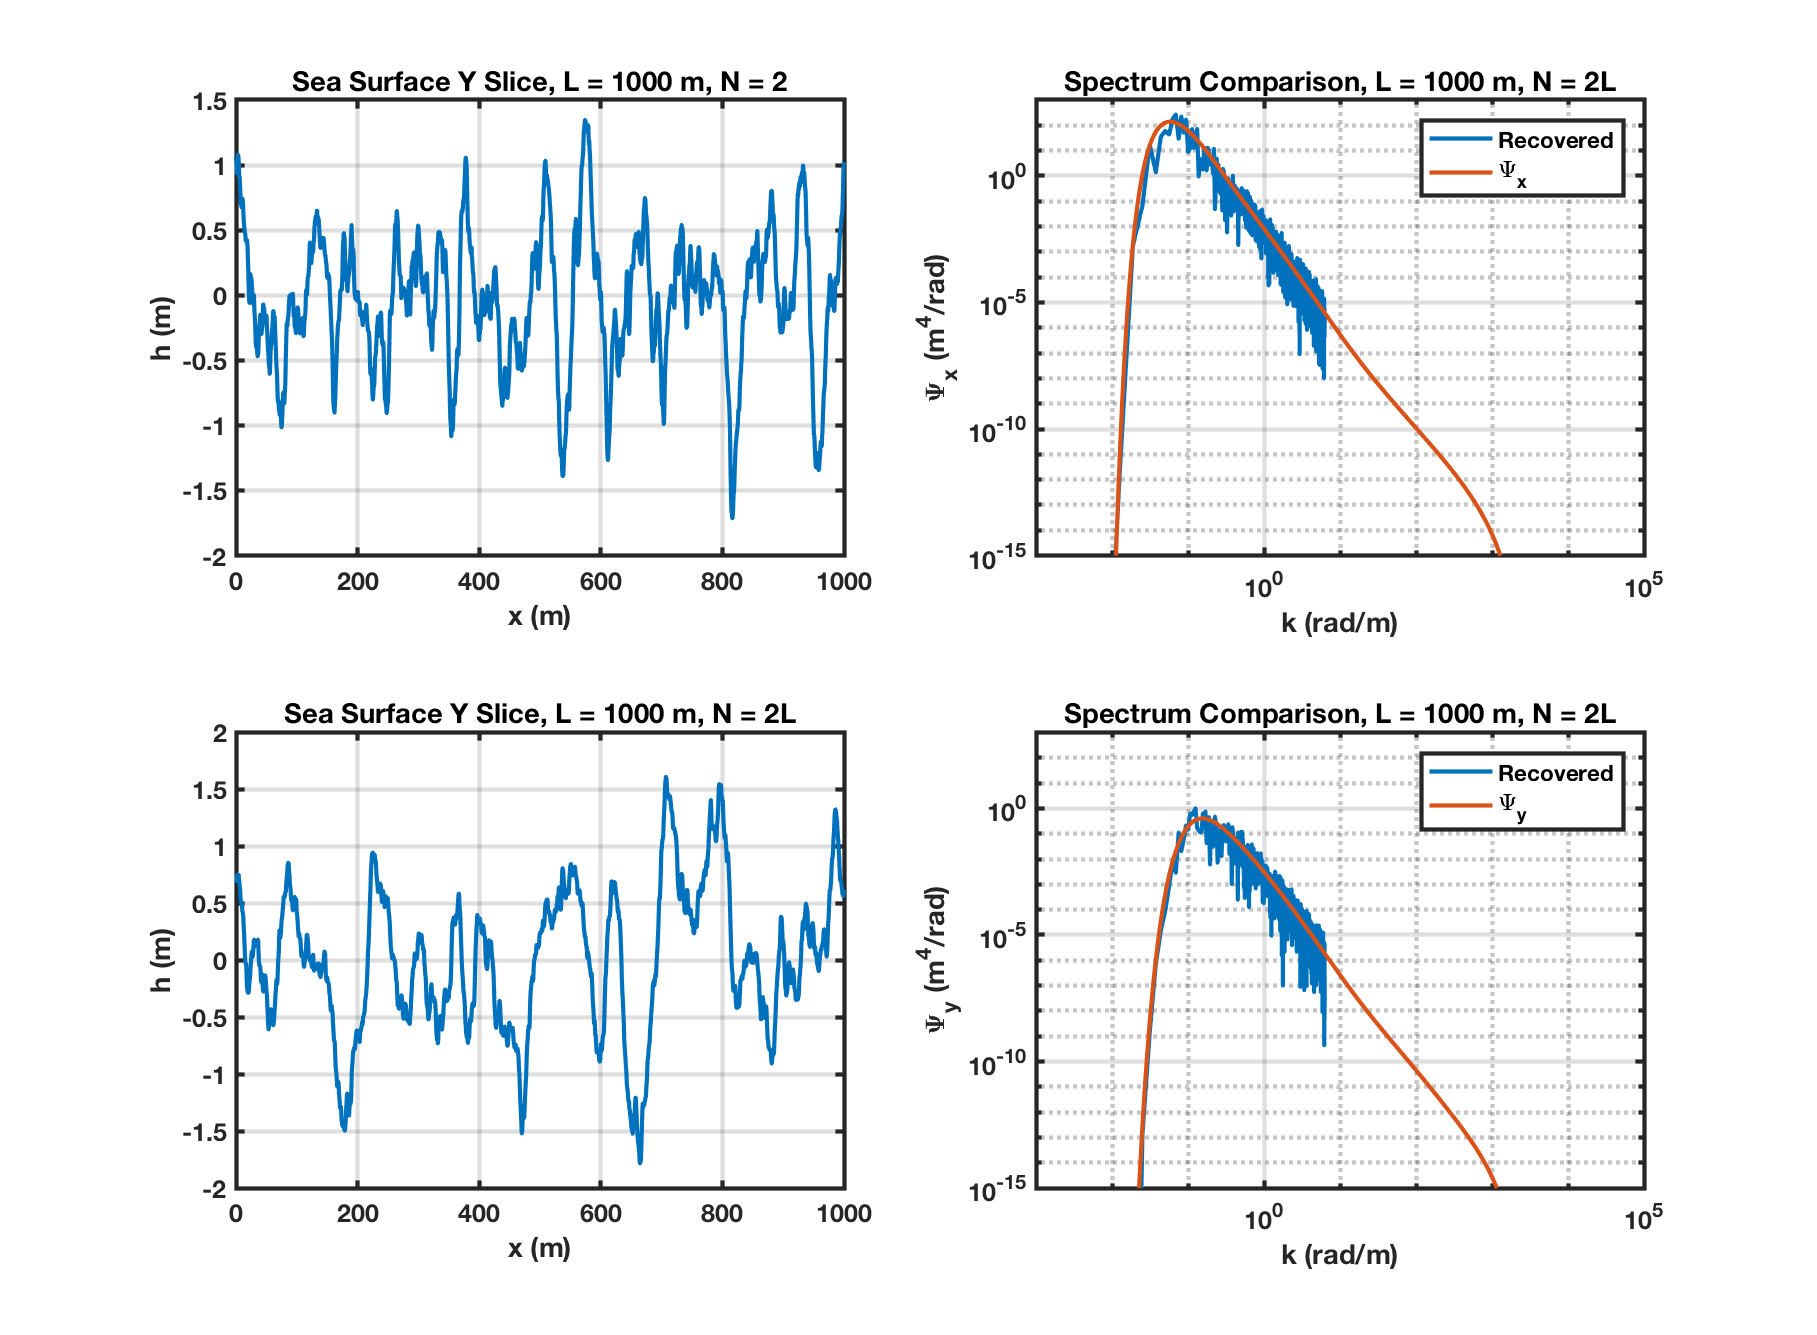
\includegraphics[width=6in]{../media/Ocean_Surface/sea_surface_2d_slices_1000.png}
  \end{center}
  \renewcommand{\baselinestretch}{1} \small\normalsize
  \begin{quote}
    \caption[X and Y Slices of 2D Generated Sea Surface, $L$ = 1 km]{X and Y Slices of 2D Generated Sea Surface, $L$ = 1 km\label{os_fig:10}}
  \end{quote}
\end{figure}
\renewcommand{\baselinestretch}{2} \small\normalsize

Figure \ref{os_fig:10a} shows the same thing as Figure \ref{os_fig:10} but with $N=10L$ instead of $N = 2L$.
\begin{figure}[H]
  \begin{center}
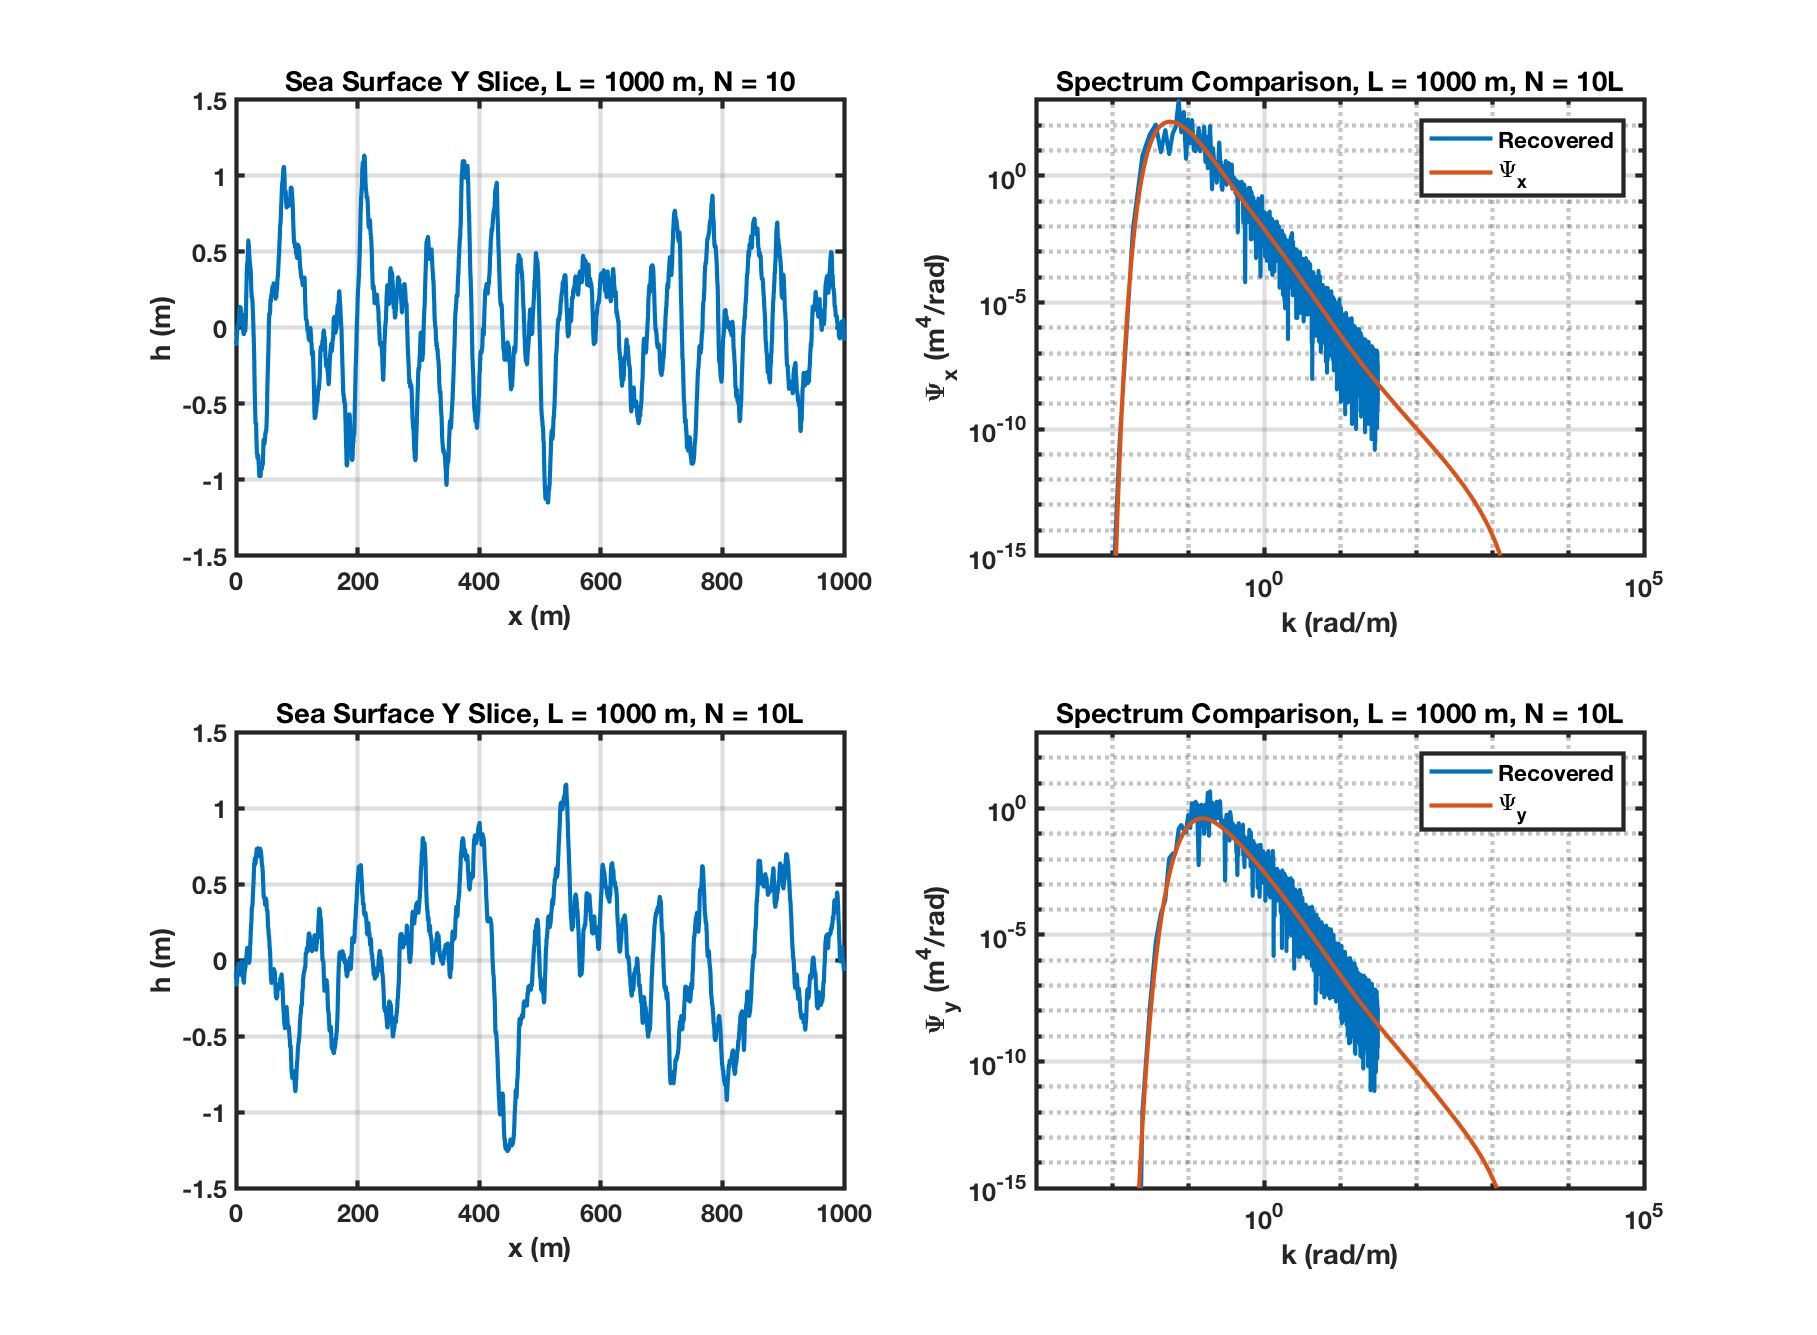
\includegraphics[width=6in]{../media/Ocean_Surface/sea_surface_2d_slices_1000_10.png}
  \end{center}
  \renewcommand{\baselinestretch}{1} \small\normalsize
  \begin{quote}
    \caption[X and Y Slices of 2D Generated Sea Surface, $L$ = 1 km, $N$ = 5$L$]{X and Y Slices of 2D Generated Sea Surface, $L$ = 1 km, $N$ = 5$L$\label{os_fig:10a}}
  \end{quote}
\end{figure}
\renewcommand{\baselinestretch}{2} \small\normalsize

For the $L$ = 5 km, $N$ = $2L$, and $U_{10}$ = 10 m/s case, Figure \ref{os_fig:11a} shows slices along the $N/2$ element in both the $x$ and $y$ planes on the left hand side and a comparison of the spectral slices in the 2-D Elfouhaily spectrum on the right hand side.
\begin{figure}[H]
  \begin{center}
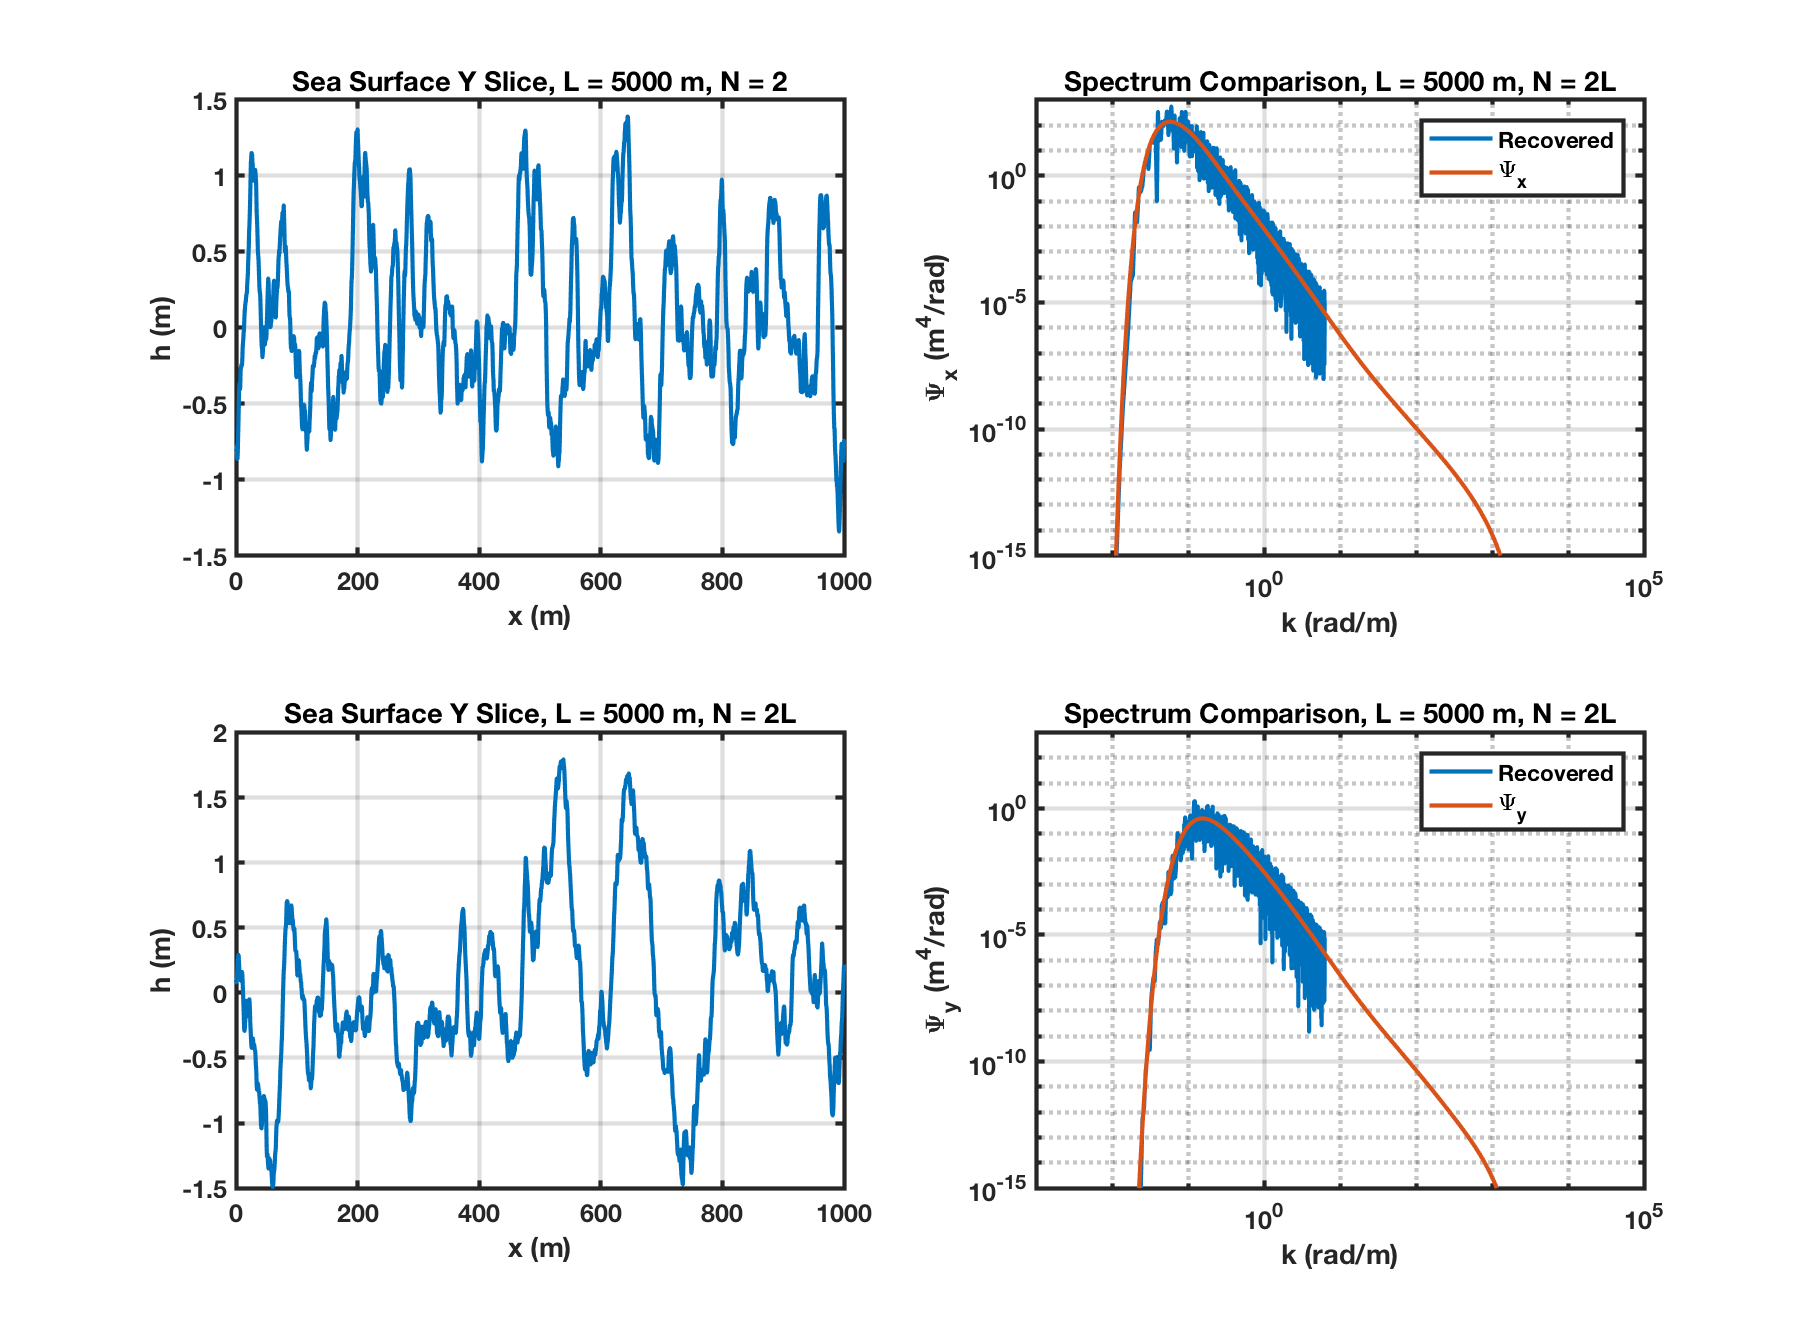
\includegraphics[width=6in]{../media/Ocean_Surface/sea_surface_2d_slices_5000.png}
  \end{center}
  \renewcommand{\baselinestretch}{1} \small\normalsize
  \begin{quote}
    \caption[X and Y Slices of 2D Generated Sea Surface, $L$ = 5 km]{X and Y Slices of 2D Generated Sea Surface, $L$ = 5 km\label{os_fig:11a}}
  \end{quote}
\end{figure}
\renewcommand{\baselinestretch}{2} \small\normalsize
 
For the $L$ = 7.5 km, $N$ = $2L$, and $U_{10}$ = 10 m/s case, Figure \ref{os_fig:12a} shows slices along the $N/2$ element in both the $x$ and $y$ planes on the left hand side and a comparison of the spectral slices in the 2-D Elfouhaily spectrum on the right hand side.
\begin{figure}[H]
  \begin{center}
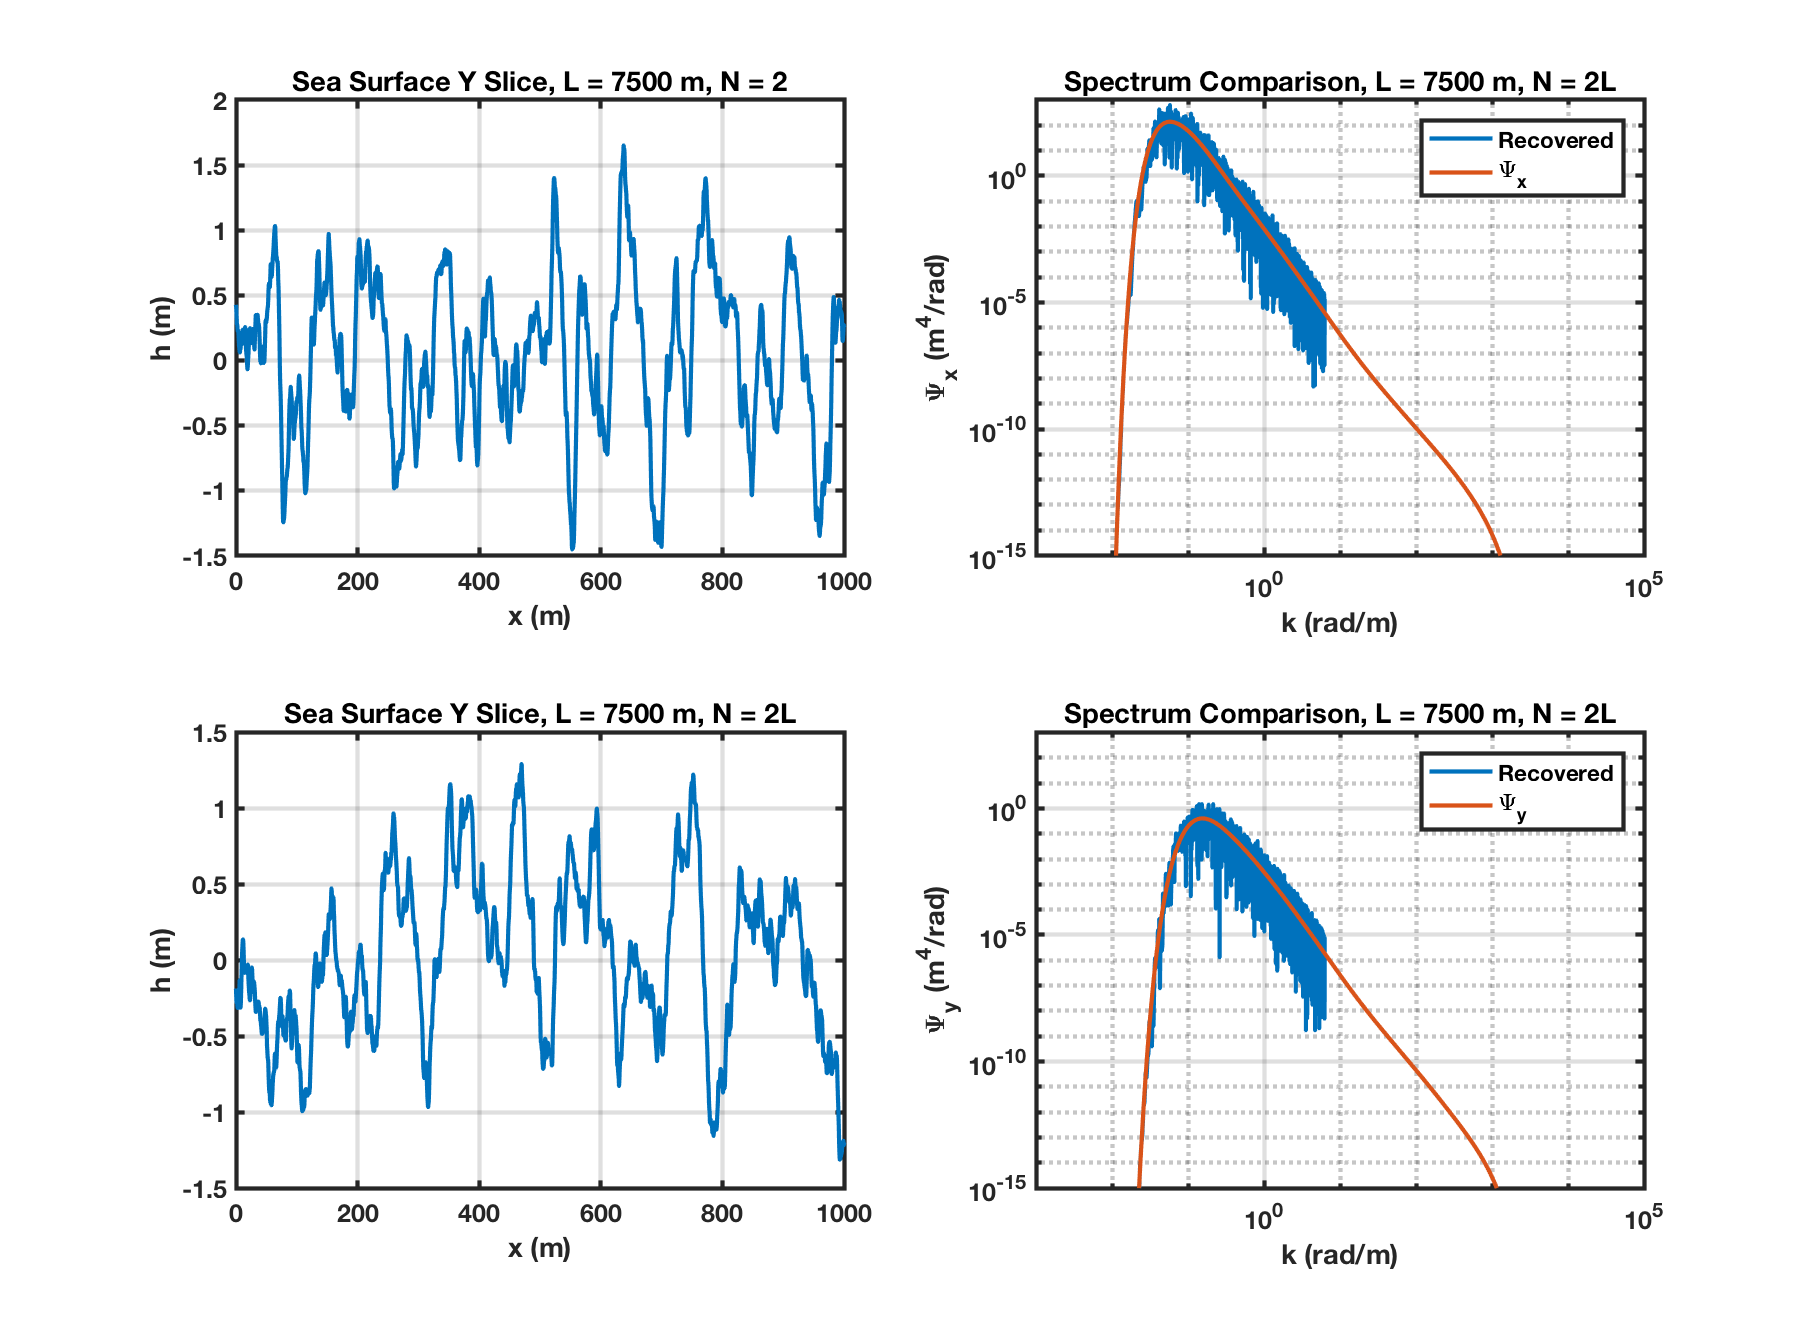
\includegraphics[width=6in]{../media/Ocean_Surface/sea_surface_2d_slices_7500.png}
  \end{center}
  \renewcommand{\baselinestretch}{1} \small\normalsize
  \begin{quote}
    \caption[X and Y Slices of 2D Generated Sea Surface, $L$ = 7.5 km]{X and Y Slices of 2D Generated Sea Surface, $L$ = 7.5 km\label{os_fig:12a}}
  \end{quote}
\end{figure}
\renewcommand{\baselinestretch}{2} \small\normalsize